\chapter{Progettazione del Sistema}
Al fine di garantire una corretta memorizzazione delle informazioni e l'esecuzione di query efficienti in tempo reale, l'architettura del sistema viene modellata seguendo un approccio \textit{orientato agli oggetti (OO).} 

%INSERISCI CLASS DIAGRAM 
\section*{Class Diagram }
\addcontentsline{toc}{section}{Class Diagram}
In particolare, il Diagramma delle Classi (\textit{Class Diagram}) definisce l'architettura statica del software secondo i paradigmi della \textit{programmazione Object-Oriented (OOP)}. All'interno di tale diagramma vengono strutturate le classi relative alla gestione dei vari profili d'accesso presenti nel sistema.
\begin{figure}[H]
    \centering
    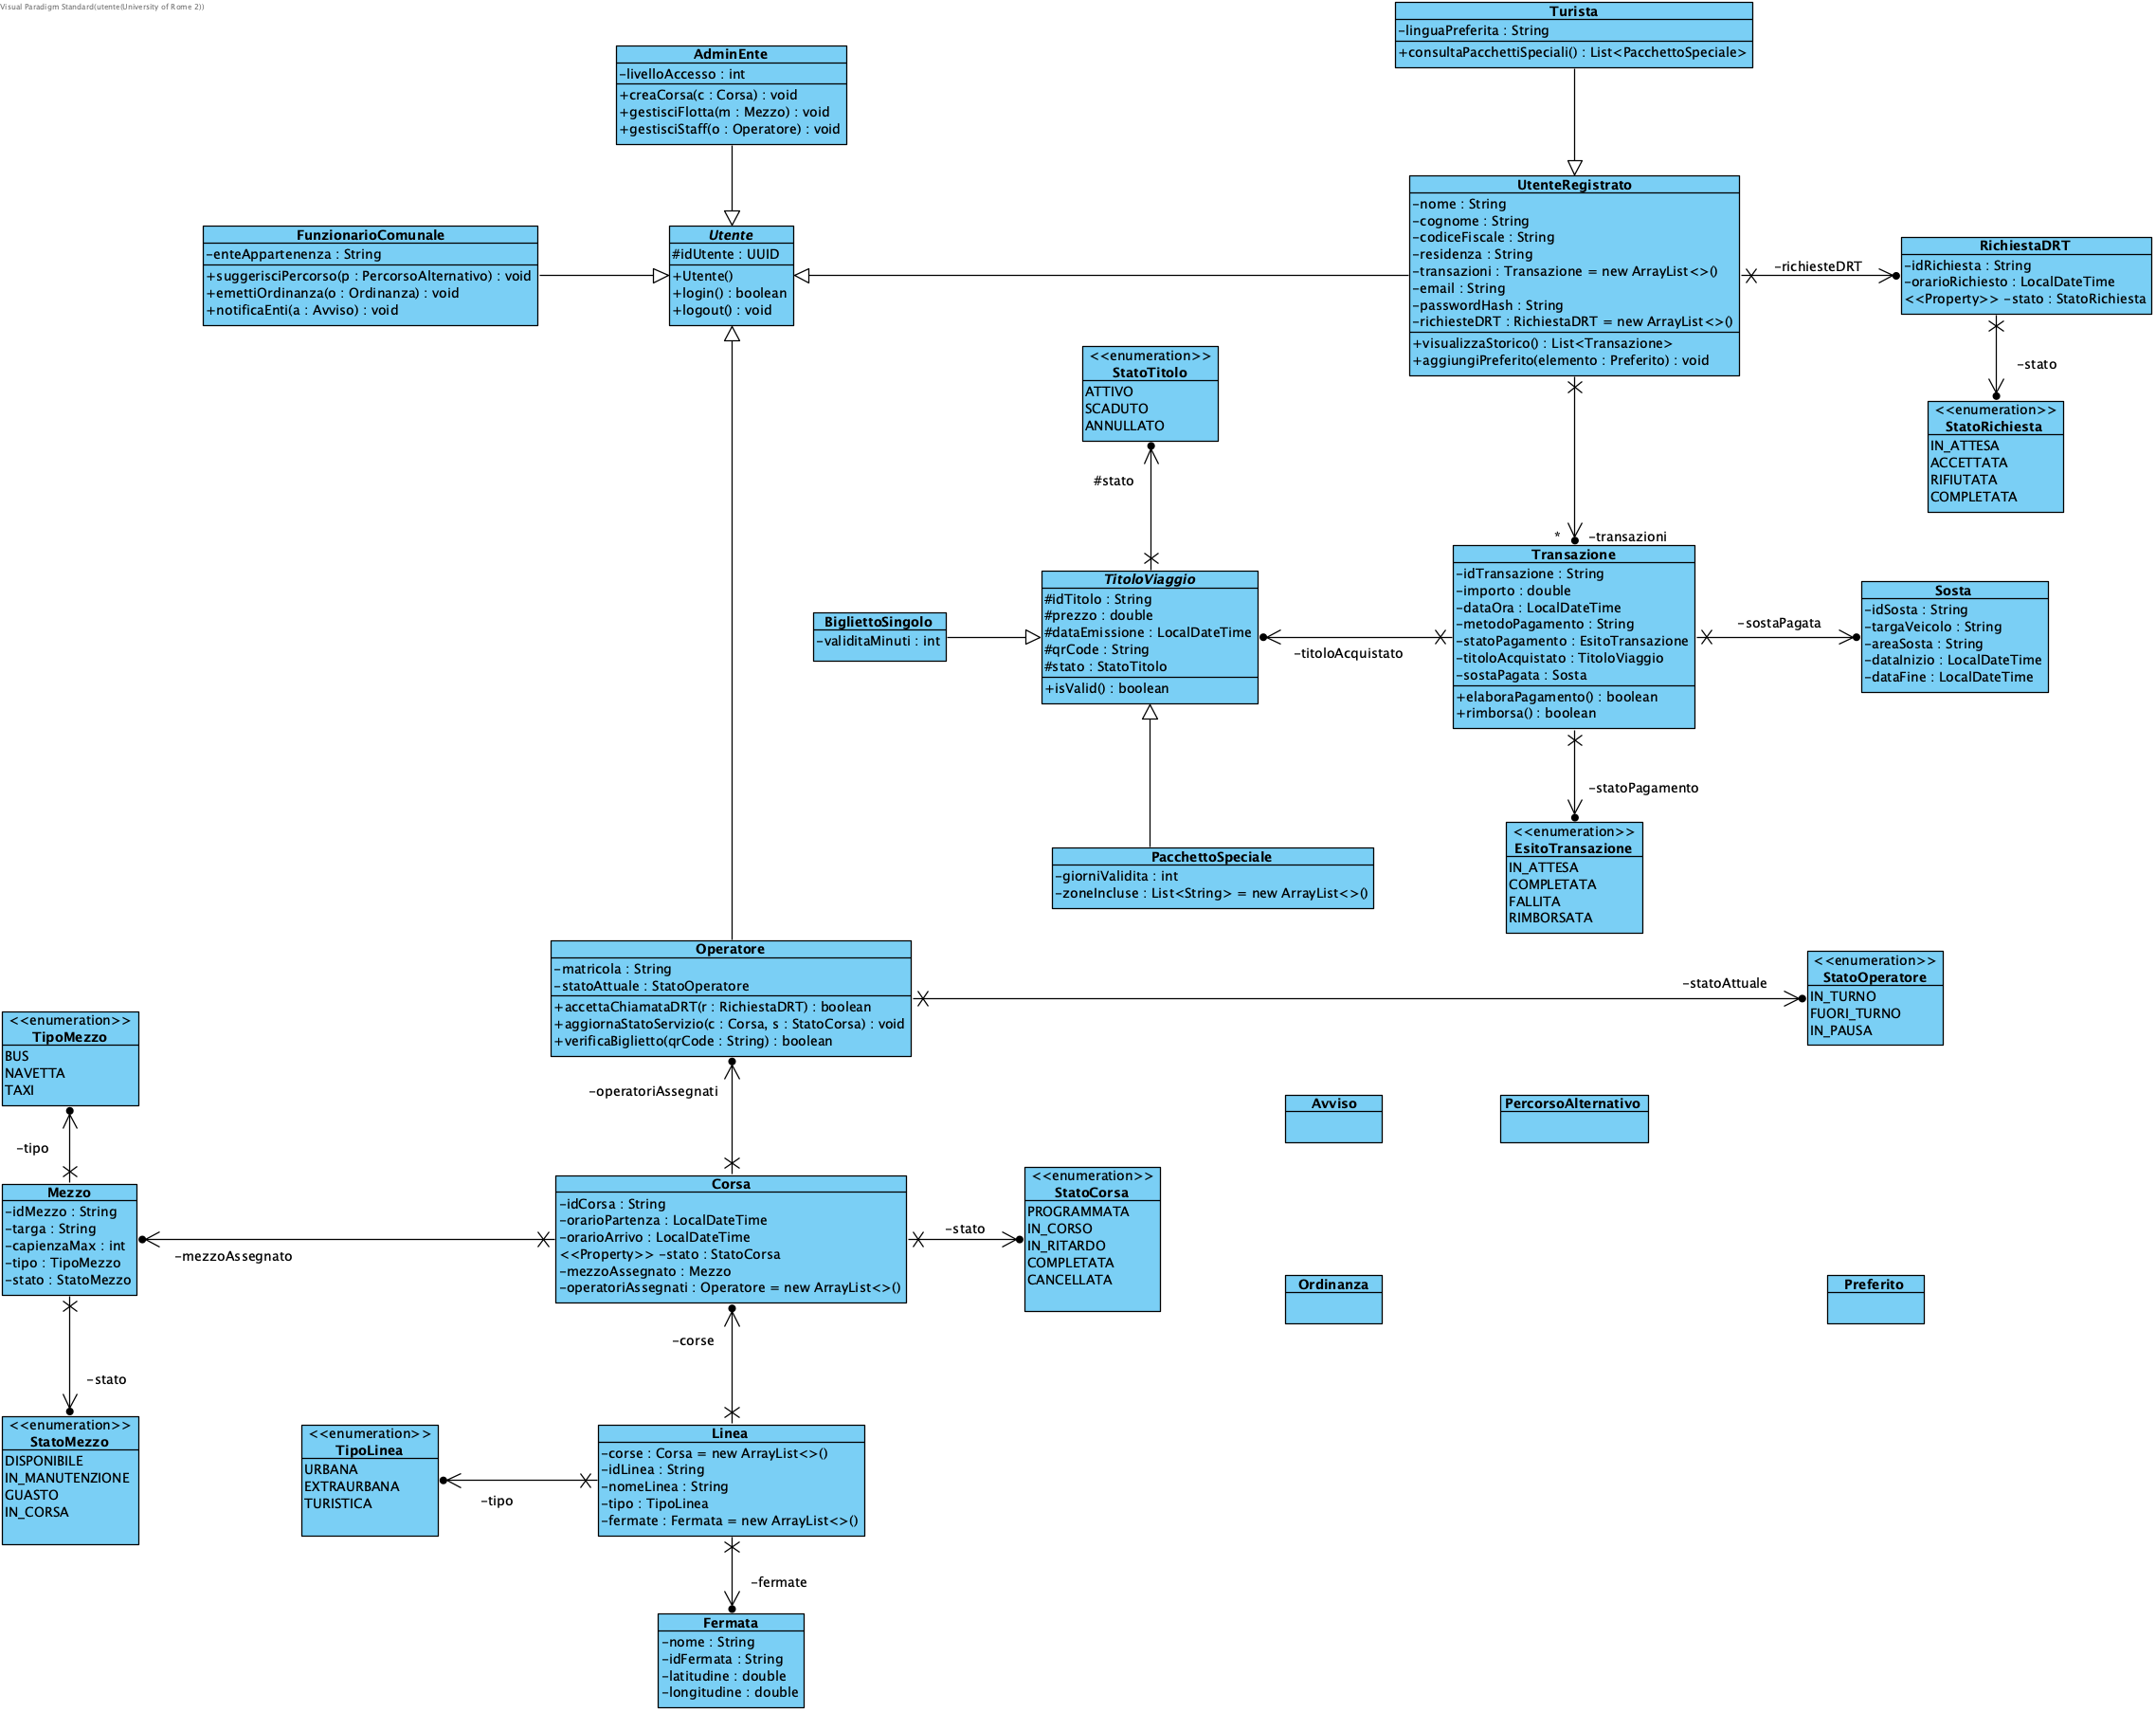
\includegraphics[width=\linewidth]{Class Diagram/Class Diagram4.png}
    \caption{}
    \label{fig:placeholder}
\end{figure}

%INSERISCI ACTIVITY DIAGRAM 
\newpage
\section*{Activity Diagram }
\addcontentsline{toc}{section}{Activity Diagram}
Infine, studiamo i \textit{diagrammi di attività} (detti anche \textit{Activity Diagram}). \\
Questi vengono utilizzati per descrivere le singole fasi dei processi interni più complessi. Nel nostro scenario, l'activity diagram modellerà il comportamento del sistema attraverso molteplici contesti operativi. Per rendere l'analisi più chiara e strutturata, ho deciso di suddividere la modellazione dei flussi di lavoro in base ai principali attori che interagiscono con la piattaforma e ai moduli di sistema più critici.

% SEZIONE UTENTE REGISTRATO

\subsection*{Azioni dell'Utente Registrato}
Il primo attore preso in esame è l'Utente Registrato. \\ Questo attore, è colui che andrà ad usare il software frequentemente per i propri spostamenti quotidiani. \\
Il suo ingresso nel sistema è regolato dal flusso di autenticazione e recupero credenziali, modellato in Figura \ref{fig:ur_auth}.

\begin{figure}[H]
    \centering
    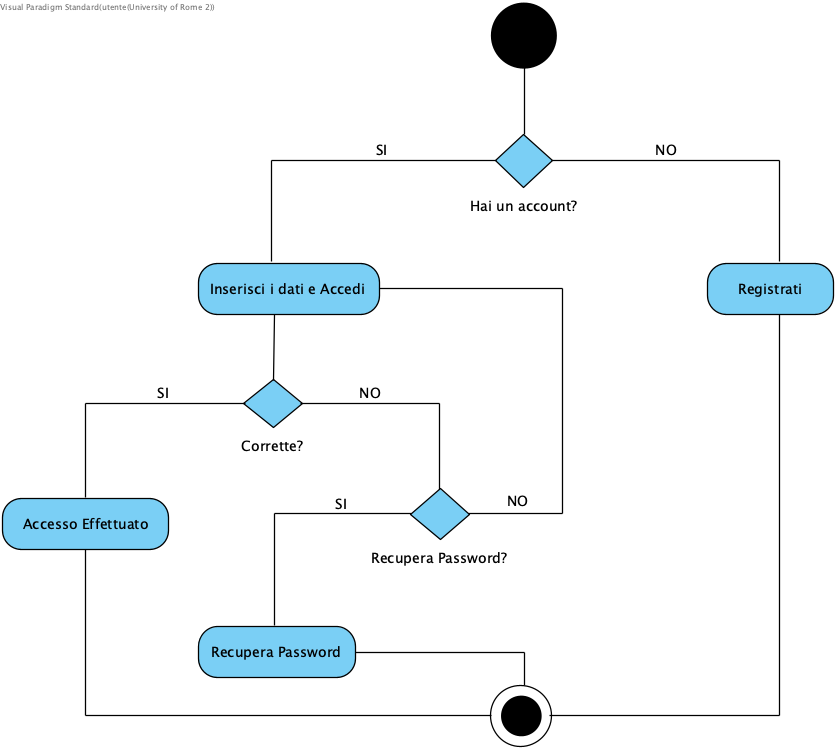
\includegraphics[width=0.8\textwidth]{Activity Diagram/Utente_Registrato/Utente_Registrato_(Autenticazione).png}
    \caption{}
    \label{fig:ur_auth}
\end{figure}
\vspace{1em}
\noindent
Una delle operazioni più frequenti compiute da questo utente è la ricerca di percorsi. \\ Accedendo al portale, egli può inserire i parametri di viaggio desiderati e avviare una ricerca iterativa fino all'individuazione di una soluzione valida (Figura \ref{fig:ur_mobilita}). A supporto di questa funzionalità, ho inserito una logica di salvataggio (Figura \ref{fig:ur_preferiti}): l'utente può aggiungere o rimuovere le tratte abituali nell'area Preferiti, migliorando notevolmente l'usabilità del software.
\begin{figure}[H]
    \centering
    \begin{minipage}{0.3\textwidth}
        \centering
        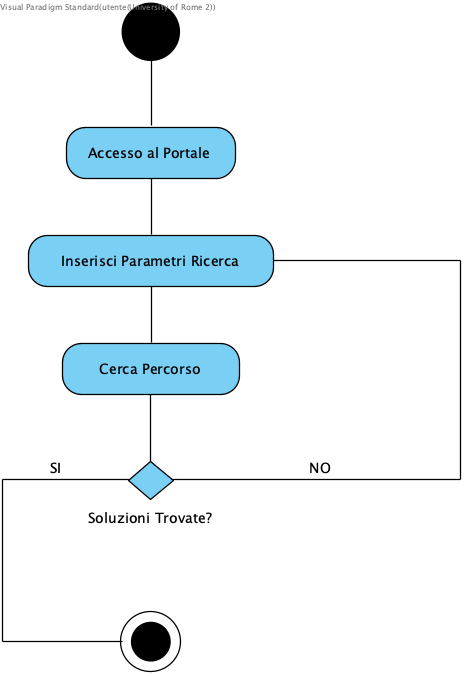
\includegraphics[width=\textwidth]{Activity Diagram/Utente_Registrato/Utente_Registrato_(Consulta MObilità).png}
        \caption{}
        \label{fig:ur_mobilita}
    \end{minipage}\hfill
    \begin{minipage}{0.6\textwidth}
        \centering
        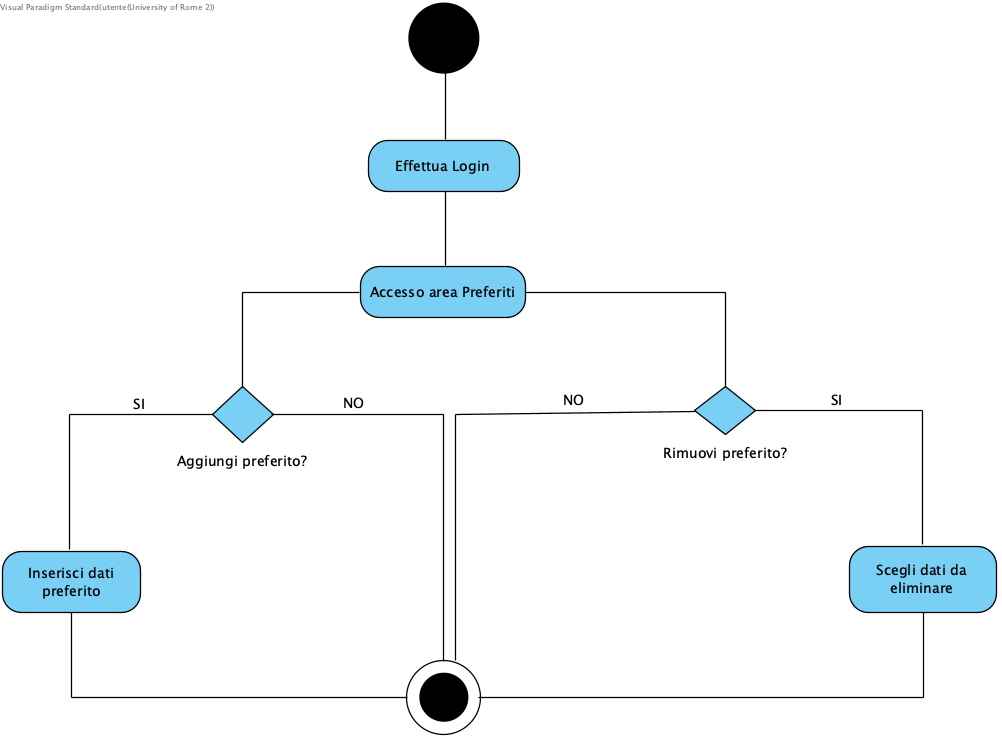
\includegraphics[width=\textwidth]{Activity Diagram/Utente_Registrato/Utente_Registarto_(Gestione_Preferiti).png}
        \caption{}
        \label{fig:ur_preferiti}
    \end{minipage}
\end{figure}
\noindent
L'applicativo gestisce in modo fluido anche i pagamenti per la sosta e il trasporto. \\ Nei diagrammi \ref{fig:ur_pag_biglietto} e \ref{fig:ur_pag_sosta} ho analizzato due scenari di acquisto molto simili ma concettualmente separati: l'acquisto di un normale biglietto (selezionando il titolo, i dati e il metodo di pagamento) e il pagamento per la sosta del proprio veicolo.
\begin{figure}[H]
    \centering
    \begin{minipage}{0.35\textwidth}
        \centering
        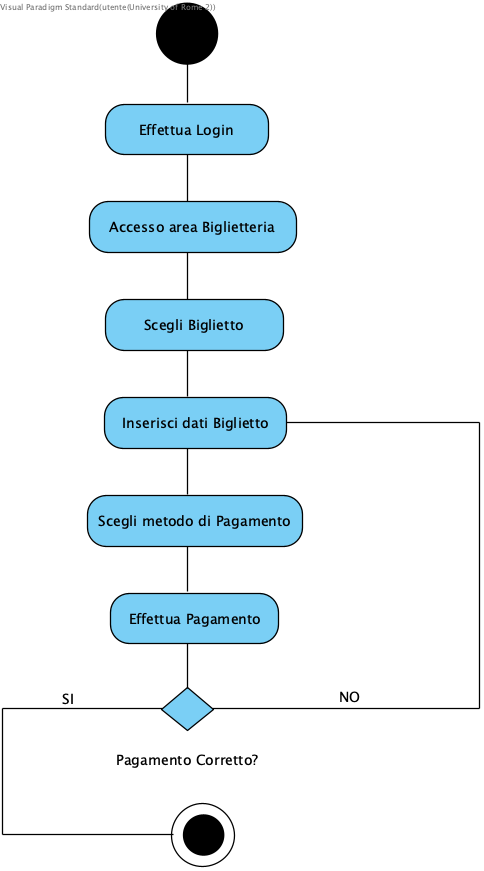
\includegraphics[width=\textwidth]{Activity Diagram/Utente_Registrato/Utente_Registrato_(Pagamento_Biglietto).png}
        \caption{}
        \label{fig:ur_pag_biglietto}
    \end{minipage}\hfill
    \begin{minipage}{0.35\textwidth}
        \centering
        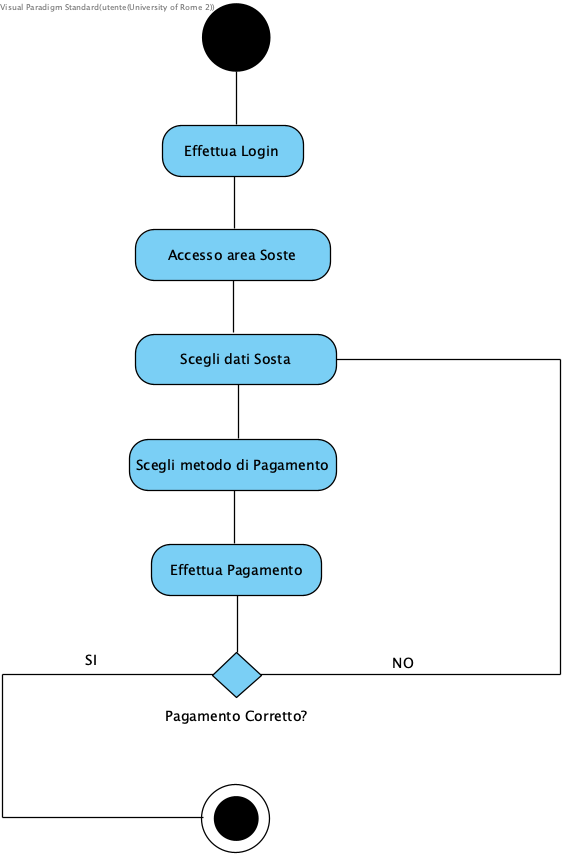
\includegraphics[width=\textwidth]{Activity Diagram/Utente_Registrato/Utente_Registrato_(Pagamento_Sosta).png}
        \caption{}
        \label{fig:ur_pag_sosta}
    \end{minipage}
\end{figure}
\noindent
Un'altra caratteristica, innovativa e molto importante che ha un impatto positivo sull'ambiente, è la prenotazione del servizio DRT (Trasporto a Chiamata). Come evidenziato in Figura \ref{fig:ur_drt}, dopo aver inserito i parametri e trovato una soluzione compatibile, l'utente seleziona le opzioni ed effettua la chiamata effettiva verso l'operatore.
\begin{figure}[H]
    \centering
    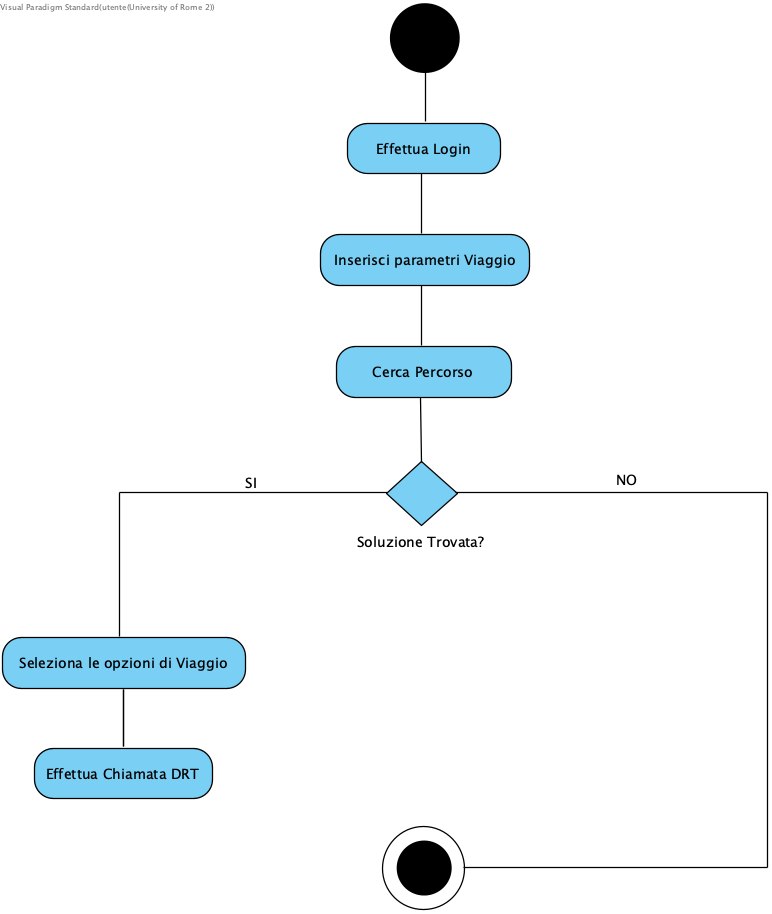
\includegraphics[width=0.45\textwidth]{Activity Diagram/Utente_Registrato/Utente_Registrato_(Prenotazione_DRT).png}
    \caption{}
    \label{fig:ur_drt}
\end{figure}
\noindent
Per concludere l'analisi di questo attore, ho modellato in Figura \ref{fig:ur_storico} la consultazione dello storico: accedendo all'area Cronologia, l'utente ha la possibilità di avere un resoconto chiaro e immediato di tutti i propri viaggi passati.
\begin{figure}[H]
    \centering
    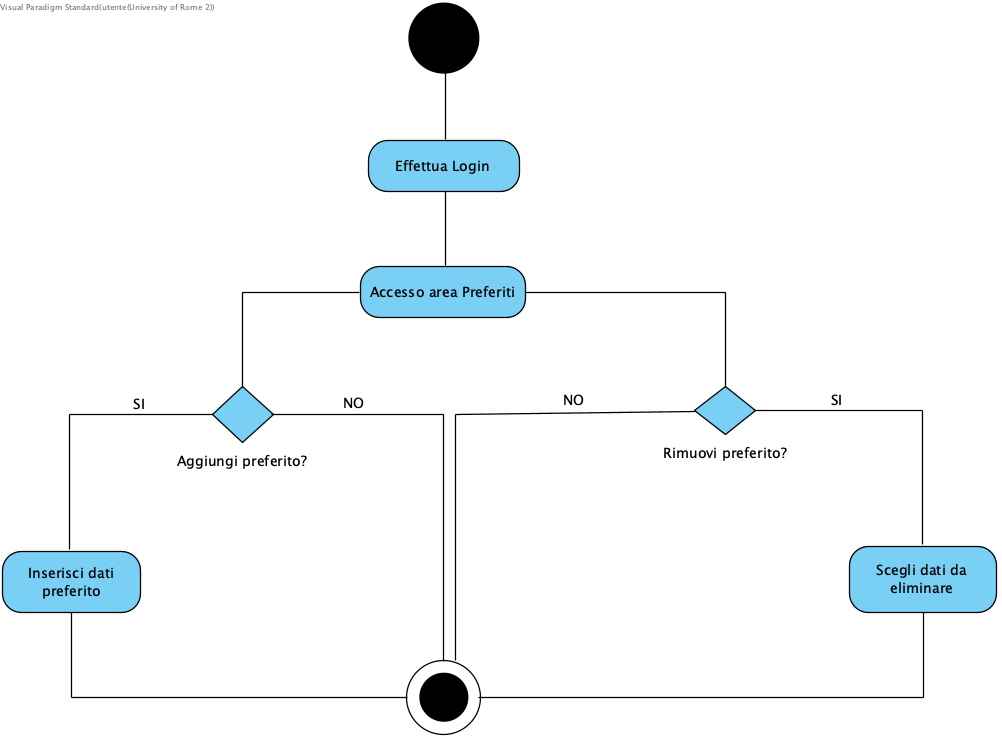
\includegraphics[width=0.6\textwidth]{Activity Diagram/Utente_Registrato/Utente_Registarto_(Gestione_Preferiti).png}
    \caption{}
    \label{fig:ur_storico}
\end{figure}

\newpage
% SEZIONE UTENTE NON REGISTRATO
\subsection*{Azioni dell'Utente Non Registrato}
A seguire, ho ritenuto opportuno descrivere anche il comportamento dell'utente il quale naviga sulla piattaforma senza possedere un account. \\
L'utente non registrato ha un accesso limitato, ma può comunque usufruire di alcune funzionalità per disporre in parte del servizio, come la consultazione della mobilità. \\ Come illustrato in Figura \ref{fig:unreg_mobilita}, il visitatore accede al portale, inserisce i parametri di ricerca e il sistema valuta iterativamente se esistono soluzioni di viaggio conformi ai criteri immessi.
\begin{figure}[H]
    \centering
    \includegraphics[width=0.25\textwidth]{Activity Diagram/Utente_non_Registrato/Utente_non_Registrato_(Consulta MObilità) copia.png}
    \caption{}
    \label{fig:unreg_mobilita}
\end{figure}
\noindent
Qualora l'utente decidesse di voler sfruttare tutte le potenzialità del sistema può attivare il processo di registrazione (Figura \ref{fig:unreg_registrazione}). Il flusso prevede la compilazione di un form e un ciclo di verifica fino alla corretta sottomissione dei dati.
\begin{figure}[H]
    \centering
    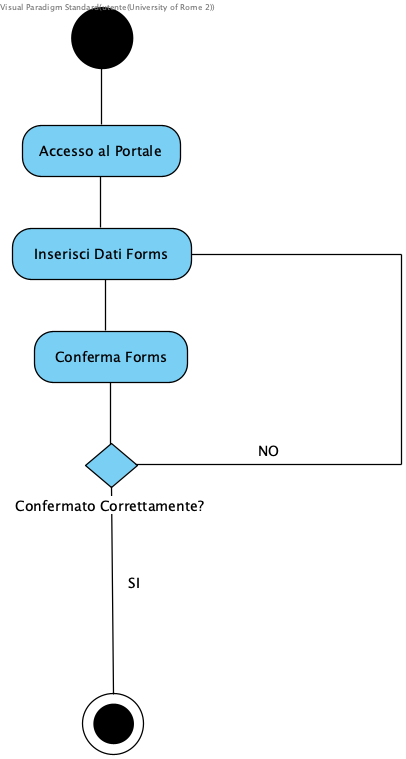
\includegraphics[width=0.25\textwidth]{Activity Diagram/Utente_non_Registrato/Utente_non_Registrato_(Registrazione).png}
    \caption{}
    \label{fig:unreg_registrazione}
\end{figure}
\newpage
% SEZIONE TURISTA
\subsection*{Azioni del Turista}
L'ultimo attore che usa il software come "consumatore" è il Turista. \\ Una volta effettuato l'accesso, l'interesse principale di questo attore è esplorare l'offerta di mobilità dedicata e acquistare i titoli di viaggio. Il flusso di consultazione è estremamente lineare: come mostrato in Figura \ref{fig:turista_consultazione}, l'utente accede all'area biglietteria ed esamina i pacchetti speciali disponibili.
\begin{figure}[H]
    \centering
    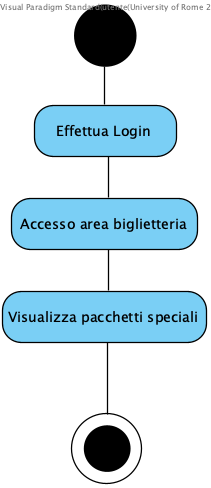
\includegraphics[width=0.2\textwidth]{Activity Diagram/Turista/Turista_(Consultazione_pacchetti).png}
    \caption{}
    \label{fig:turista_consultazione}
\end{figure}
\vspace{1em}
\noindent
Se il turista decide di procedere con l'acquisto di un pacchetto, il diagramma di attività si espande (Figura \ref{fig:turista_acquisto}). Dopo aver selezionato il pacchetto di interesse, l'utente procede all'inserimento dei dati di fatturazione fino al raggiungimento di un esito positivo della transazione.
\begin{figure}[H]
    \centering
    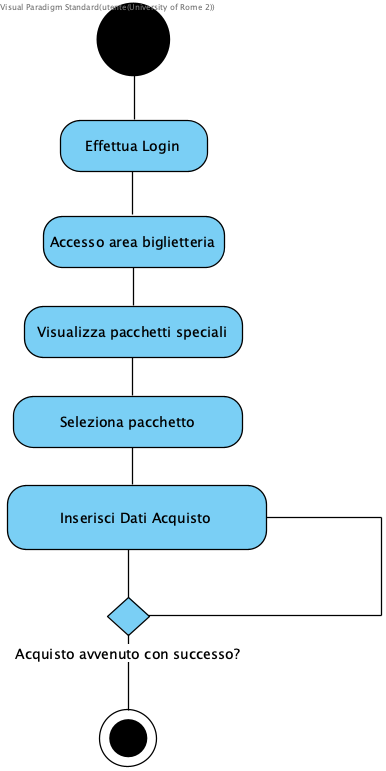
\includegraphics[width=0.25\textwidth]{Activity Diagram/Turista/Turista_(Acquista_Pacchetti).png}
    \caption{}
    \label{fig:turista_acquisto}
\end{figure}
\newpage
% SEZIONE ADMIN ENTE
\subsection*{Azioni dell'Admin Ente}
Spostandoci ora sul lato gestionale della piattaforma, analizziamo l'Admin dell'Ente. \\ Come per ogni utente del sistema, il primo passo fondamentale è l'autenticazione. Il diagramma in Figura \ref{fig:admin_auth} mostra il flusso decisionale che porta al login, alla registrazione o al recupero della password in caso di credenziali errate.
\begin{figure}[H]
    \centering
    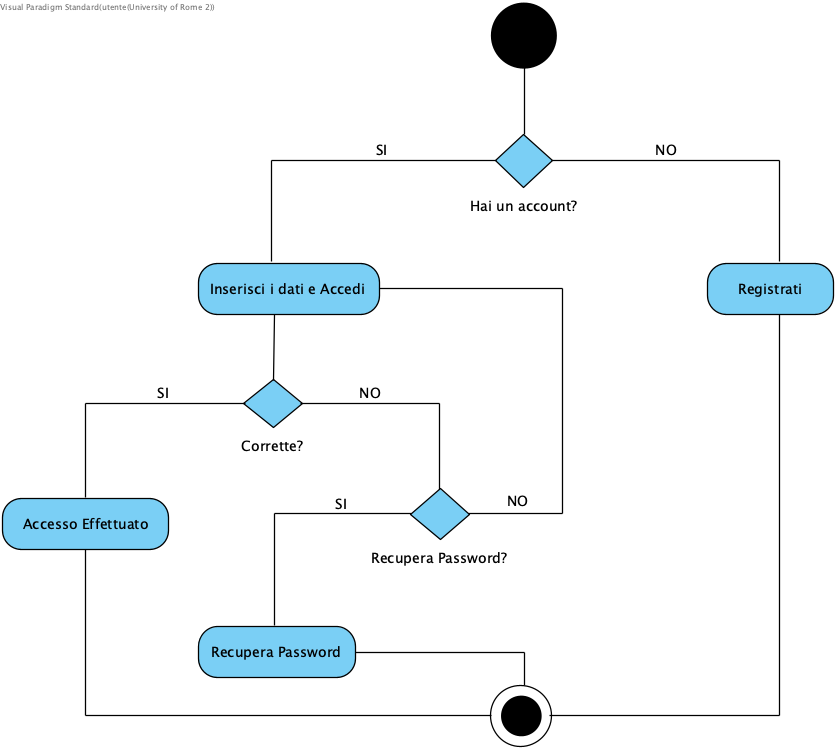
\includegraphics[width=0.5\textwidth]{Activity Diagram/Admin_Ente/Admin_Ente_(Autenticazione).png}
    \caption{}
    \label{fig:admin_auth}
\end{figure}
\noindent
Una volta effettuato l'accesso, l'Admin accede al Pannello di Mobilità. \\ Come illustrato in Figura \ref{fig:admin_pannello}, da questo snodo centrale l'utente può diramarsi in quattro attività principali: la gestione delle corse, della flotta, delle tariffe e dello staff. Ogni operazione prevede una fase di salvataggio e la possibilità di tornare al pannello principale per avviare una nuova attività.
\begin{figure}[H]
    \centering
    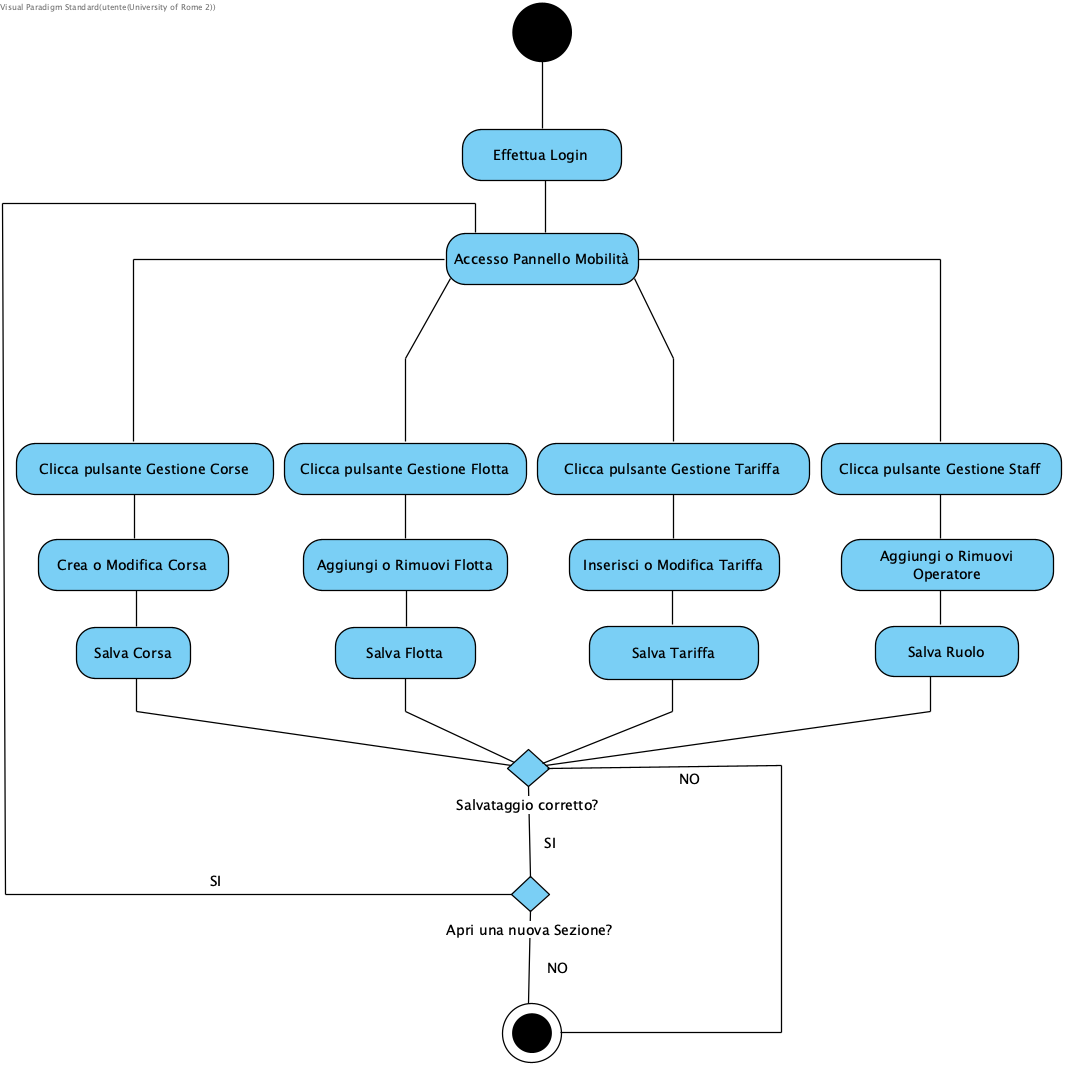
\includegraphics[width=0.5\textwidth]{Activity Diagram/Admin_Ente/Admin_Ente_(Gestione_Pannello_Mobilità).png}
    \caption{}
    \label{fig:admin_pannello}
\end{figure}
\newpage
% SEZIONE OPERATORE
\subsection*{Azioni dell'Operatore}
Un altro attore chiave della componente gestionale e operativa sul campo è l'Operatore, il quale interagisce con la piattaforma per le proprie mansioni quotidiane. Il suo flusso di autenticazione segue la logica standard del sistema (Figura \ref{fig:op_auth}).
\begin{figure}[H]
    \centering
    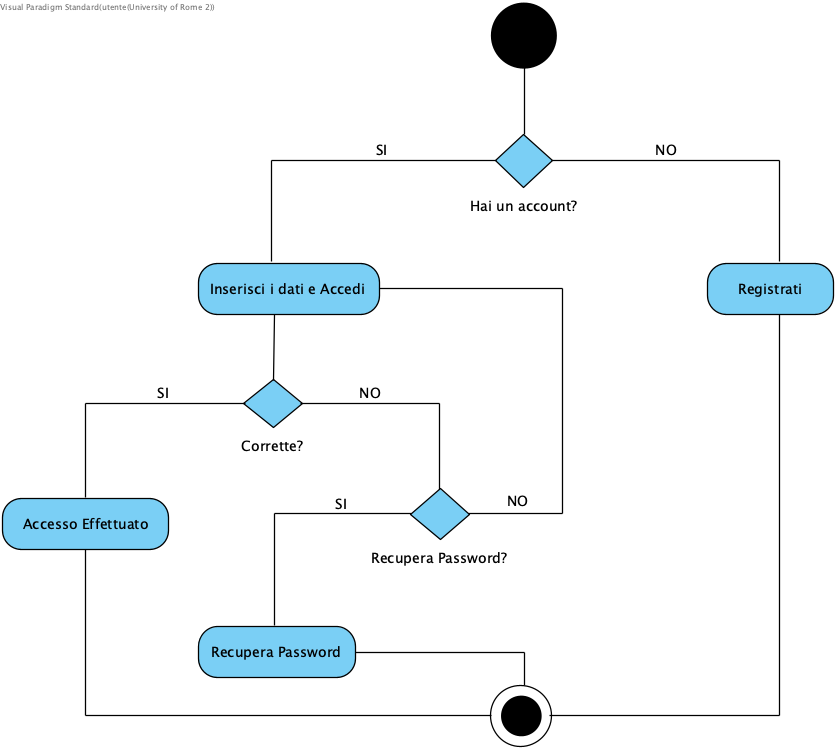
\includegraphics[width=0.5\textwidth]{Activity Diagram/Operatore/Operatore_(Autenticazione).png}
    \caption{}
    \label{fig:op_auth}
\end{figure}
\noindent
Nel contesto dei servizi di trasporto a chiamata (DRT), l'operatore riceve notifiche per nuove corse. Come vediamo in Figura \ref{fig:op_drt} vi è una semplice diramazione logica tra l'accettazione o il rifiuto della chiamata da parte dell'autista.
\begin{figure}[H]
    \centering
    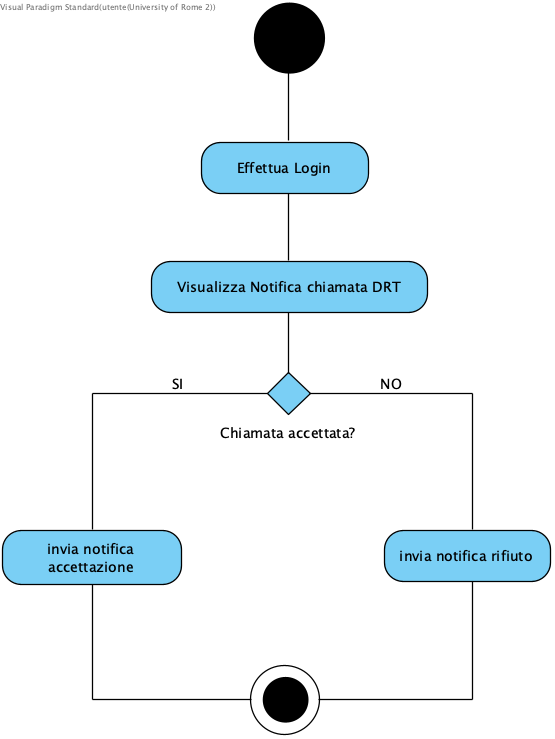
\includegraphics[width=0.3\textwidth]{Activity Diagram/Operatore/Operatore_(Gestione corse_DRT).png}
    \caption{}
    \label{fig:op_drt}
\end{figure}
\noindent
Una delle azioni più importanti dell'Operatore è quella di mantenere aggiornato lo stato del servizio. L'Activity Diagram in Figura \ref{fig:op_stato} mostra il processo ciclico di inserimento e caricamento dei dati aggiornati nell'area di servizio.
\begin{figure}[H]
    \centering
    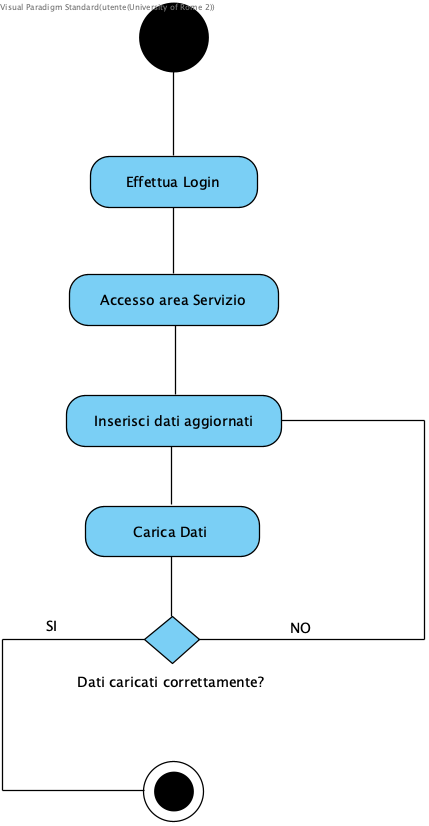
\includegraphics[width=0.3\textwidth]{Activity Diagram/Operatore/Operatore_(Stato_Servizio).png}
    \caption{}
    \label{fig:op_stato}
\end{figure}
\noindent
L'ultima azione, non per importanza, è la verifica dei titoli di viaggio. Come si evince dalla Figura \ref{fig:op_verifica}, l'operatore scannerizza il QRCode del biglietto. Se la lettura fallisce o il codice non è valido visivamente, il sistema offre un flusso alternativo permettendo l'inserimento manuale del codice.
\begin{figure}[H]
    \centering
    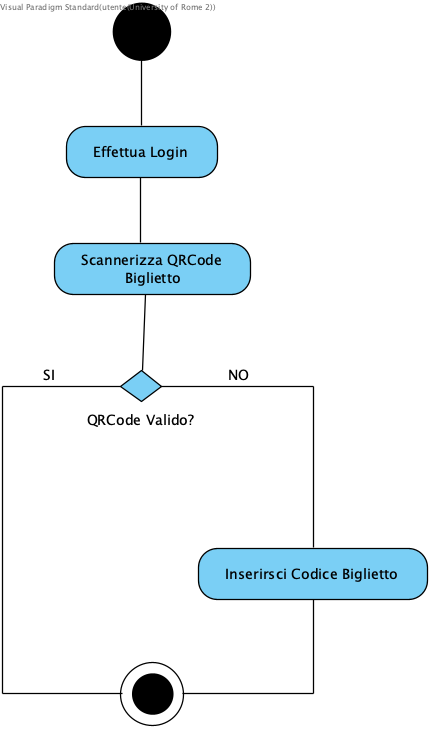
\includegraphics[width=0.3\textwidth]{Activity Diagram/Operatore/Operatore_(Verifica_Prenotazioni).png}
    \caption{}
    \label{fig:op_verifica}
\end{figure}
\newpage
% SEZIONE FUNZIONARIO COMUNALE
\subsection*{Azioni del Funzionario Comunale}
L'ultima figura che gestisce, stavolta dal punto di vista istituzionale, il software è il  Funzionario Comunale. Quest'ultimo ha un ruolo legato alla gestione degli avvisi e della viabilità cittadina. Il flusso parte regolarmente con l'autenticazione al portale (Figura \ref{fig:funz_auth}).
\begin{figure}[H]
    \centering
    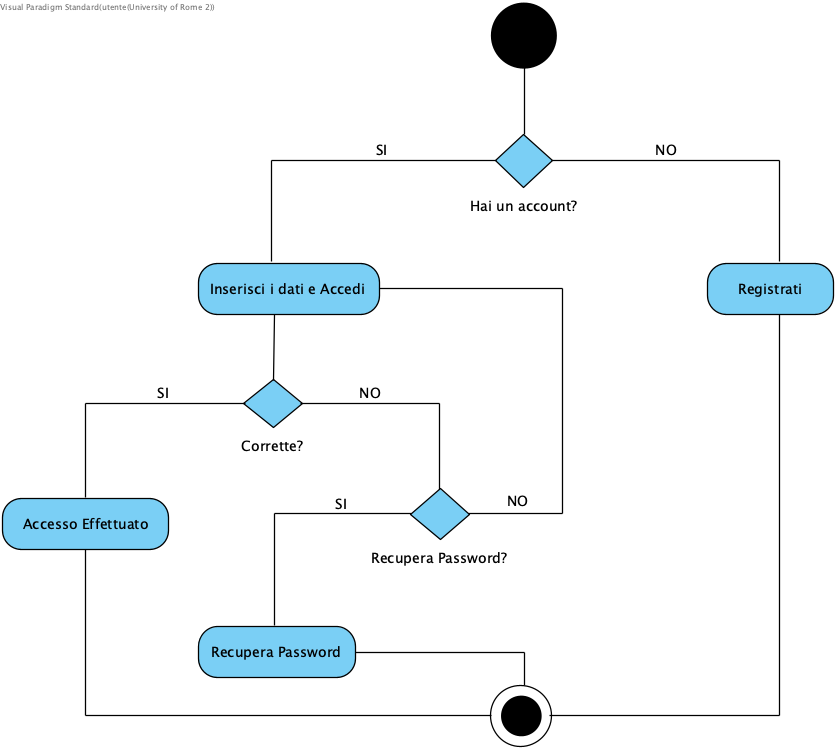
\includegraphics[width=0.5\textwidth]{Activity Diagram/Funzionario_Comunale/Funzionario_Comunale_(Autenticazione).png}
    \caption{}
    \label{fig:funz_auth}
\end{figure}
\noindent
Il funzionario ha accesso alla sezione Avvisi, dove può compiere diverse operazioni cruciali per la viabilità. La prima è la gestione delle ordinanze (Figura \ref{fig:funz_ordinanze}), che prevede il caricamento del documento e la verifica del corretto inserimento a sistema.\\
Un'altra operazione fondamentale è la comunicazione con altri enti. Come visibile in Figura \ref{fig:funz_notifica}, il funzionario può selezionare un avviso personale, scegliere l'ente destinatario, comporre un messaggio e inviarlo, con un controllo sull'esito della trasmissione.
\begin{figure}[H]
    \centering
    \begin{minipage}{0.2\textwidth}
        \centering
        \includegraphics[width=\textwidth]{"Activity Diagram/Funzionario_Comunale/Funzionario_Comunale_(Gestisce_Ordinanze).png"}
        \caption{}
        \label{fig:funz_ordinanze}
    \end{minipage}
    \hspace{3cm} 
    \begin{minipage}{0.2\textwidth}
        \centering
        \includegraphics[width=\textwidth]{"Activity Diagram/Funzionario_Comunale/Funzionario_Comunale_(Notifica_Enti).png"}
        \caption{}
        \label{fig:funz_notifica}
    \end{minipage}
\end{figure}
\noindent
Infine, per minimizzare l'impatto sul traffico durante gli eventi paesani, il funzionario può suggerire percorsi alternativi. Il diagramma in Figura \ref{fig:funz_percorsi} illustra l'inserimento dei dati relativi all'evento e il caricamento dei tracciati alternativi a sistema.
\begin{figure}[H]
    \centering
    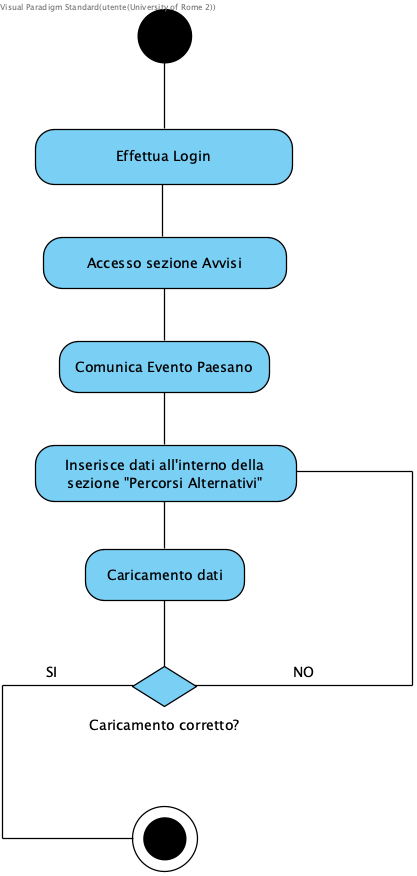
\includegraphics[width=0.4\textwidth]{Activity Diagram/Funzionario_Comunale/Funzionario_Comunale_(Suggerimento_Percorsi).png}
    \caption{}
    \label{fig:funz_percorsi}
\end{figure}
\newpage
% SEZIONE PAGAMENTI E RIMBORSI
\subsection*{Azioni del Payment}
Infine, per garantire la robustezza logica dell'intera applicazione, ho studiato i flussi relativi al modulo delle transazioni finanziarie. A differenza dei precedenti, questi diagrammi coinvolgono attivamente il backend e sistemi di terze parti (modellati tramite le \textit{partitions}). \\
La Figura \ref{fig:pay_elaborazione} mostra il processo di elaborazione dei pagamenti: il sistema riceve e controlla il formato dei dati; in caso di esito positivo, richiede l'autorizzazione a un modulo esterno o ente bancario e, all'arrivo della risposta di approvazione, aggiorna il database ed emette la ricevuta.
\begin{figure}[H]
    \centering
    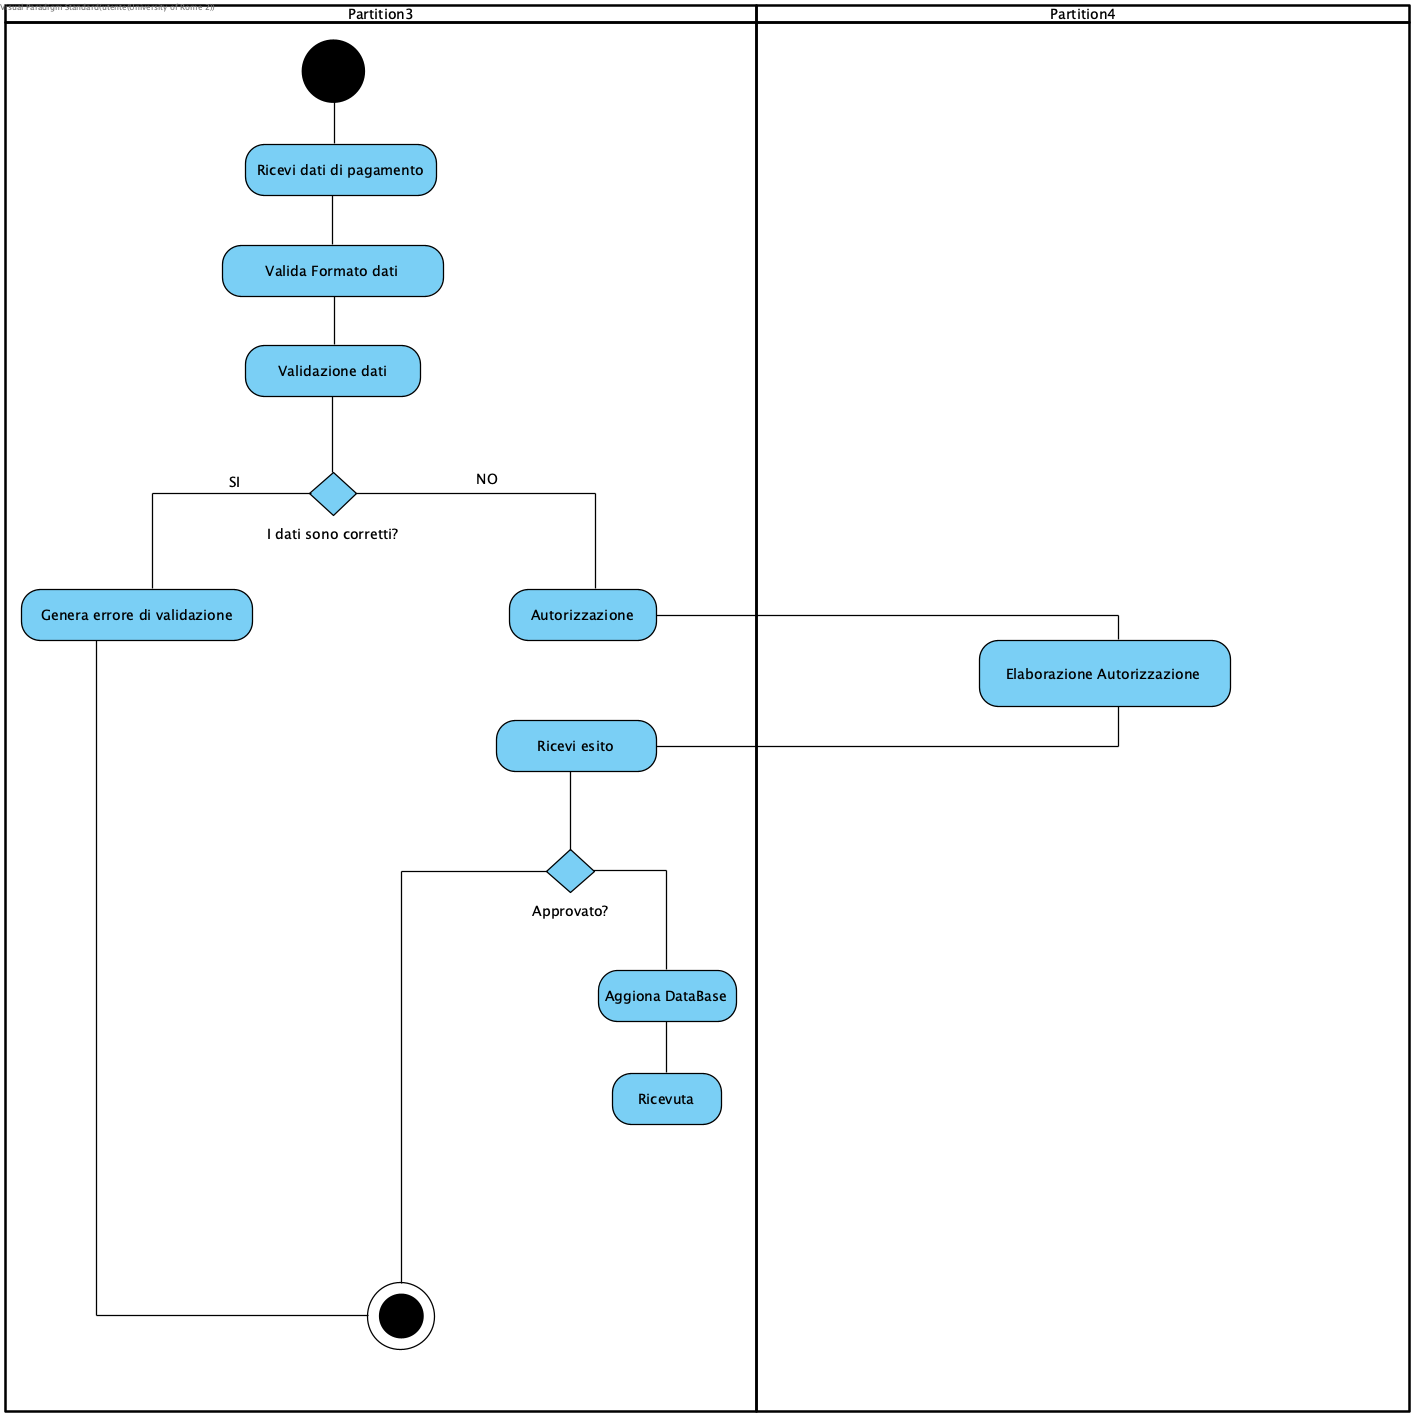
\includegraphics[width=0.4\textwidth]{Activity Diagram/Payment/Payment_(Elaborazione_Pagamenti).png}
    \caption{}
    \label{fig:pay_elaborazione}
\end{figure}
\noindent
Parallelamente, anche la gestione dei rimborsi (Figura \ref{fig:pay_rimborsi}) segue un iter di validazione rigoroso e cross-partition. A seguito di una richiesta, il sistema recupera la transazione, verifica i criteri di idoneità per il reso e, in caso positivo, elabora lo storno.
\begin{figure}[H]
    \centering
    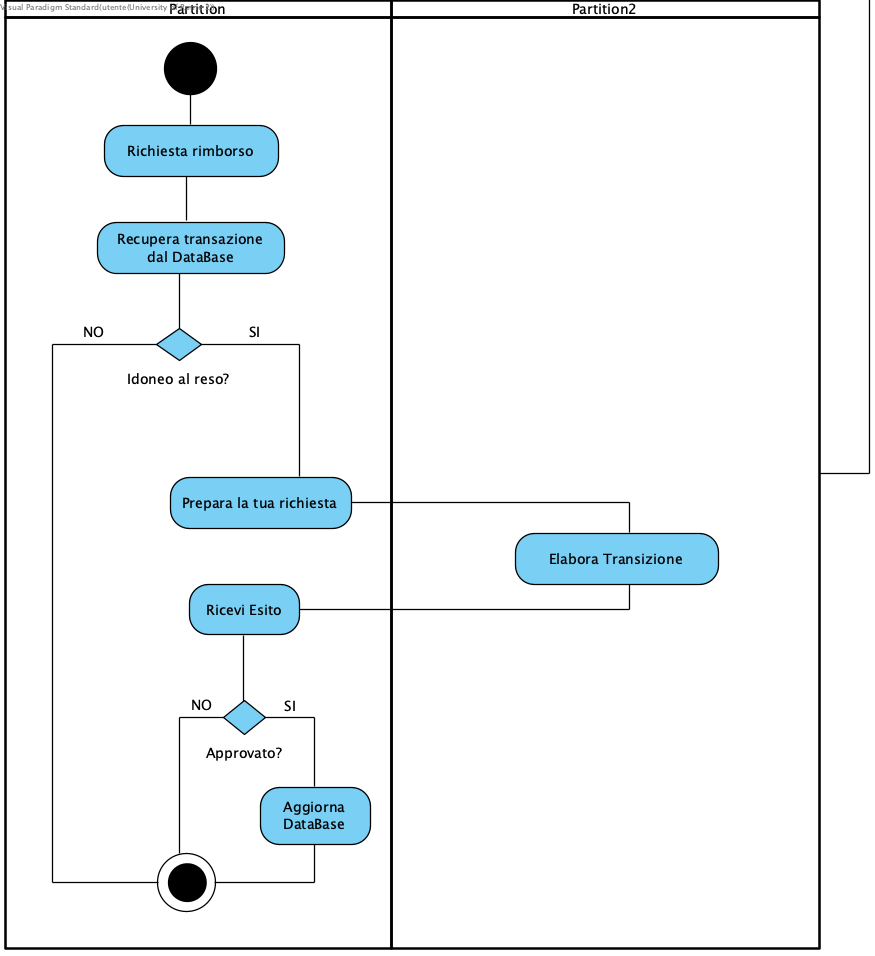
\includegraphics[width=0.4\textwidth]{Activity Diagram/Payment/Payment_(Gestione_RImborsi).png}
    \caption{}
    \label{fig:pay_rimborsi}
\end{figure}

%INSERISCI SEQUENCE DIAGRAM 
\newpage
\section*{Sequence Diagram }
\addcontentsline{toc}{section}{Sequence Diagram}
Successivamente, andremo ad analizzare i \textit{diagrammi di sequenza} (detti anche \textit{sequence diagram}).
\\
Questi catturano l'evoluzione temporale dei messaggi e delle richieste di metodi scambiati tra i vari oggetti e attori del sistema. 

% SEZIONE UTENTE REGISTRATO
\subsection*{Sequence dell'Utente Registrato}
Di seguito vengono presentati i Sequence Diagram relativi alle principali operazioni effettuate dall'attore \textbf{Utente Registrato}. Questi schemi illustrano in dettaglio come le richieste dell'utente vengano gestite dai vari componenti del sistema.
\\
Il primo processo analizzato riguarda proprio l'autenticazione, in cui l'utente inserisce le proprie credenziali, come visibile nella Figura \ref{fig:ur_auth}. Le credenziali vengono validate dal sistema: in caso di successo viene garantito l'accesso, mentre in caso di fallimento viene notificata l'assenza dell'account o avviata la procedura per il recupero della password.

\begin{figure}[H]
    \centering
    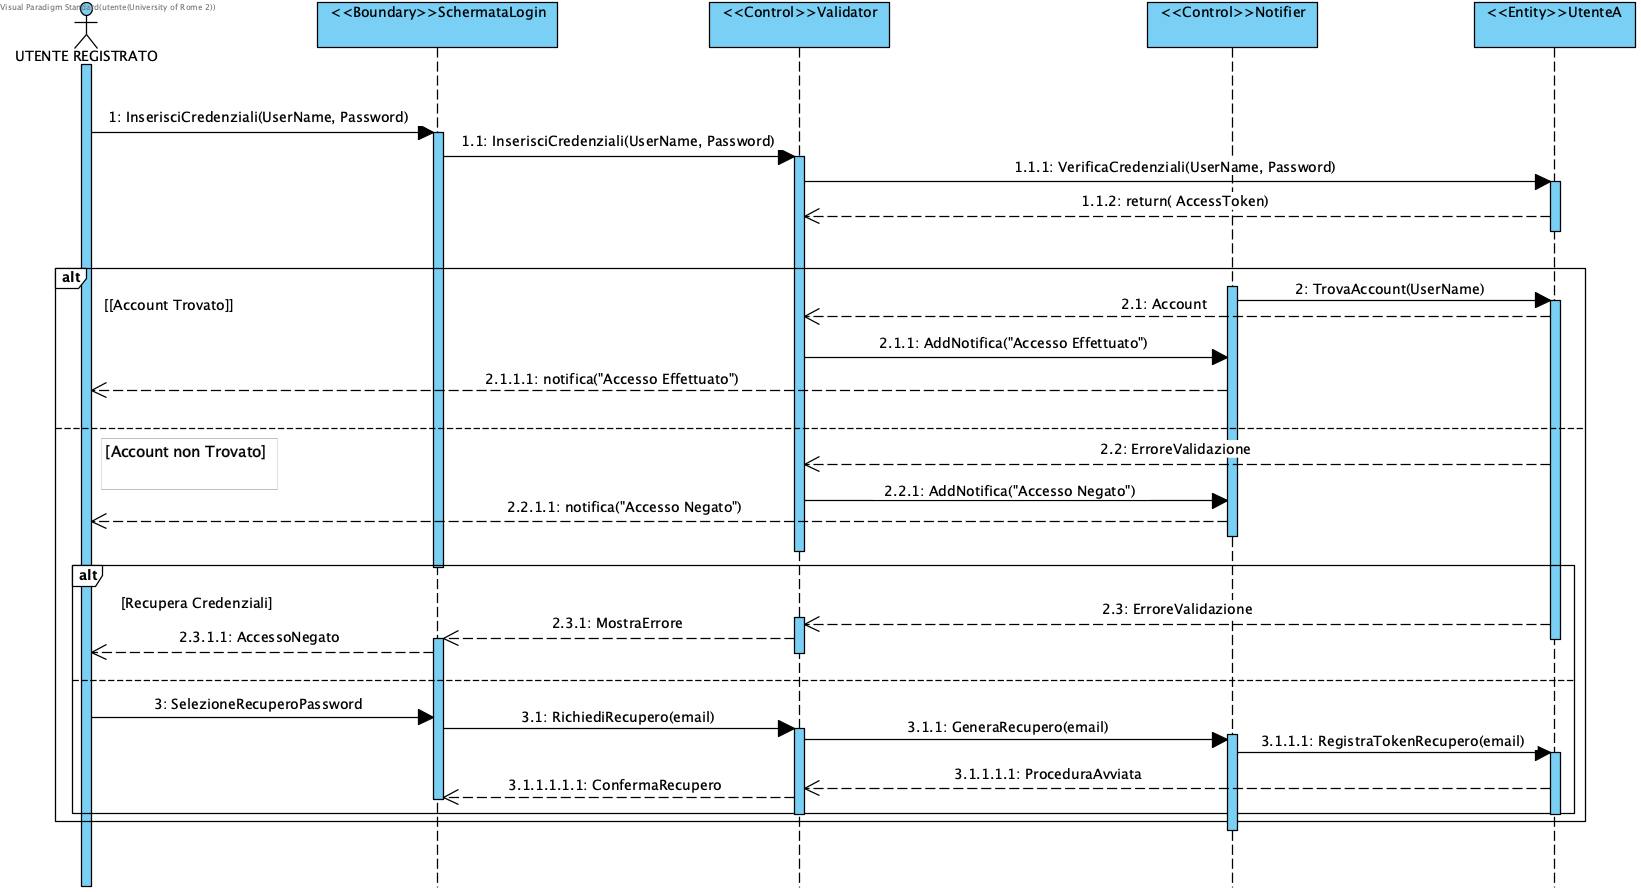
\includegraphics[width= 1.0\textwidth]{Sequence Diagram/Utente_Registrato_(Autenticazione).png}
    \caption{}
    \label{fig:ur_auth}
\end{figure}
\newpage

\noindent Una volta autenticato, l'utente può interagire con le funzionalità principali, tra cui la consultazione della mobilità. 
La seguente procedura riguarda la ricerca di una tratta (Figura \ref{fig:seq_cons}) prevedendo l'inserimento dei parametri di partenza e destinazione; se ritenuti validi dai moduli di controllo, il sistema restituisce le informazioni dettagliate su tratte, orari, fermate e stato del servizio, altrimenti richiede una correzione manuale all'utente.

\begin{figure}[H]
    \centering
    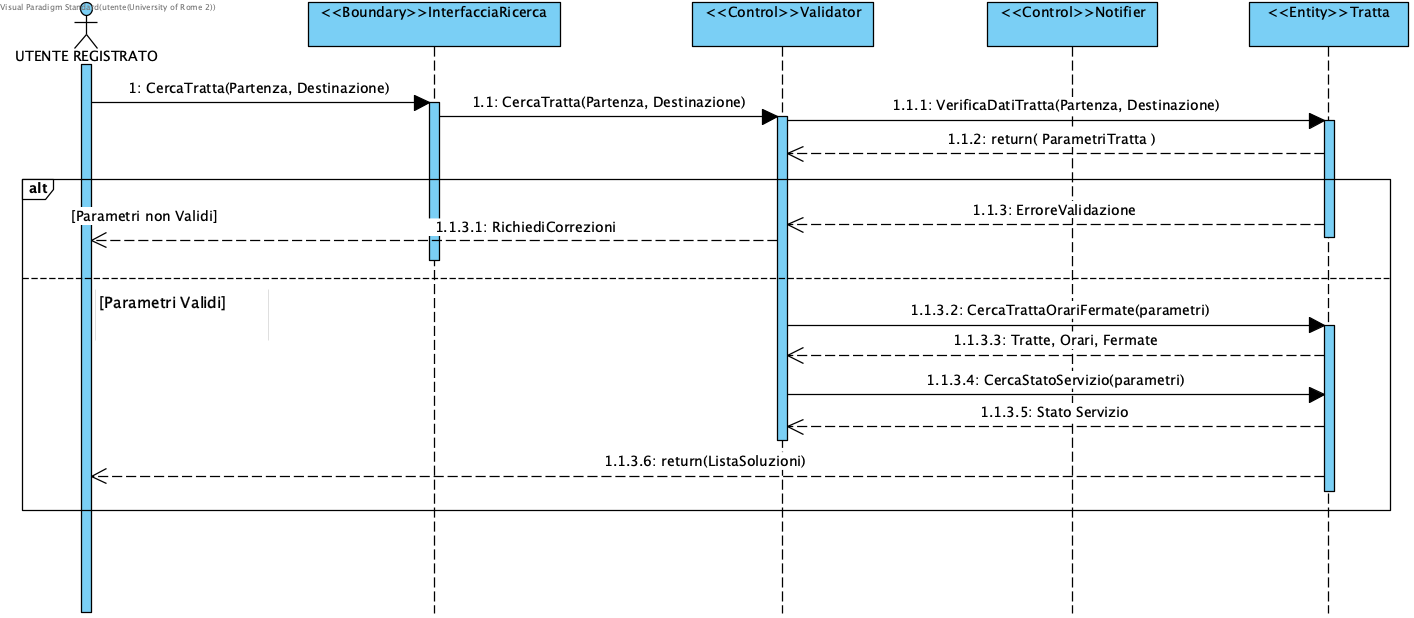
\includegraphics[width=1.0\textwidth]{Sequence Diagram/Utente_Registrato_(Consultazione_Mobilità).png}
    \caption{}
    \label{fig:seq_cons}
\end{figure}

\noindent Per agevolare l'utilizzo continuativo dell'applicazione, il sistema offre la possibilità di salvare percorsi e fermate ricorrenti. Il diagramma in Figura \ref{fig:seq_pref} mostra come l'utente possa aggiungere o rimuovere specifici elementi interfacciandosi con la schermata dedicata, la quale mantiene all'interno del sistema le tratte preferite dall'utente.

\begin{figure}[H]
    \centering
    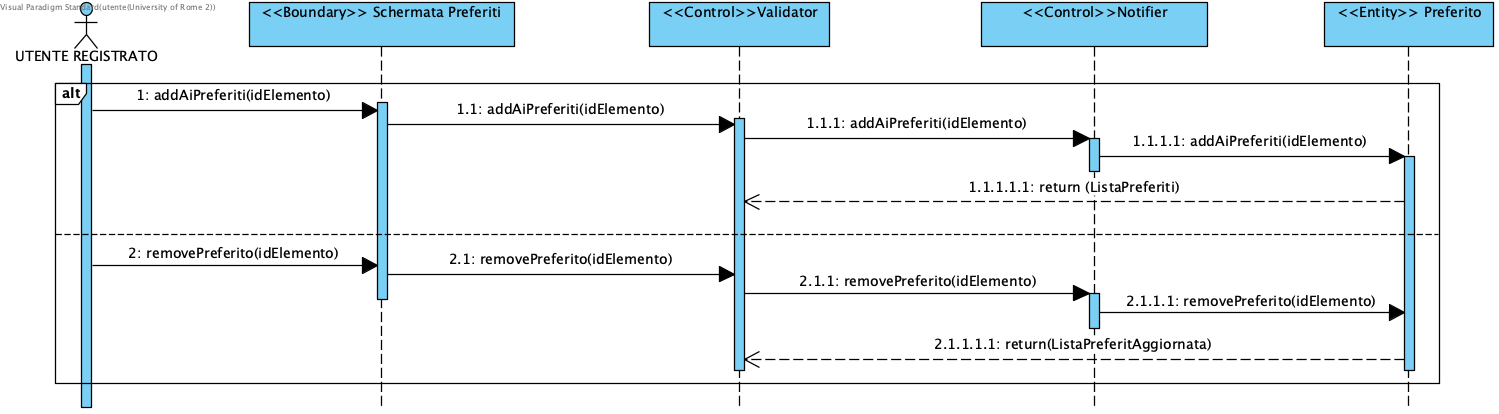
\includegraphics[width= 1.0\textwidth]{Sequence Diagram/Utente_Registro_(Gestione_Preferiti).png}
    \caption{}
    \label{fig:seq_pref}
\end{figure}
\newpage

\noindent Un aspetto cruciale dell'infrastruttura riguarda la gestione delle transazioni economiche, suddivise nell'acquisto di titoli di viaggio e nel pagamento delle soste. Nel caso dell'acquisto di un biglietto (Figura \ref{fig:seq_ticket}), il sistema elabora e valida i dati di pagamento interagendo in back-end con i componenti di controllo, generando infine una ricevuta se l'operazione va a buon fine, oppure richiedendo di modificare i dati in caso di errore.
\\
Similmente, per il pagamento di un'area di sosta, come evidenziato nella Figura \ref{fig:seq_soste}, vediamo come i dati in ingresso differiscono dal precedente sequence (infatti i nuovi dati sono: targa, orari, area specifica), ma la validazione e la notifica dell'esito della transazione mantengono la medesima coerenza architetturale.

\begin{figure}[H]
    \centering
    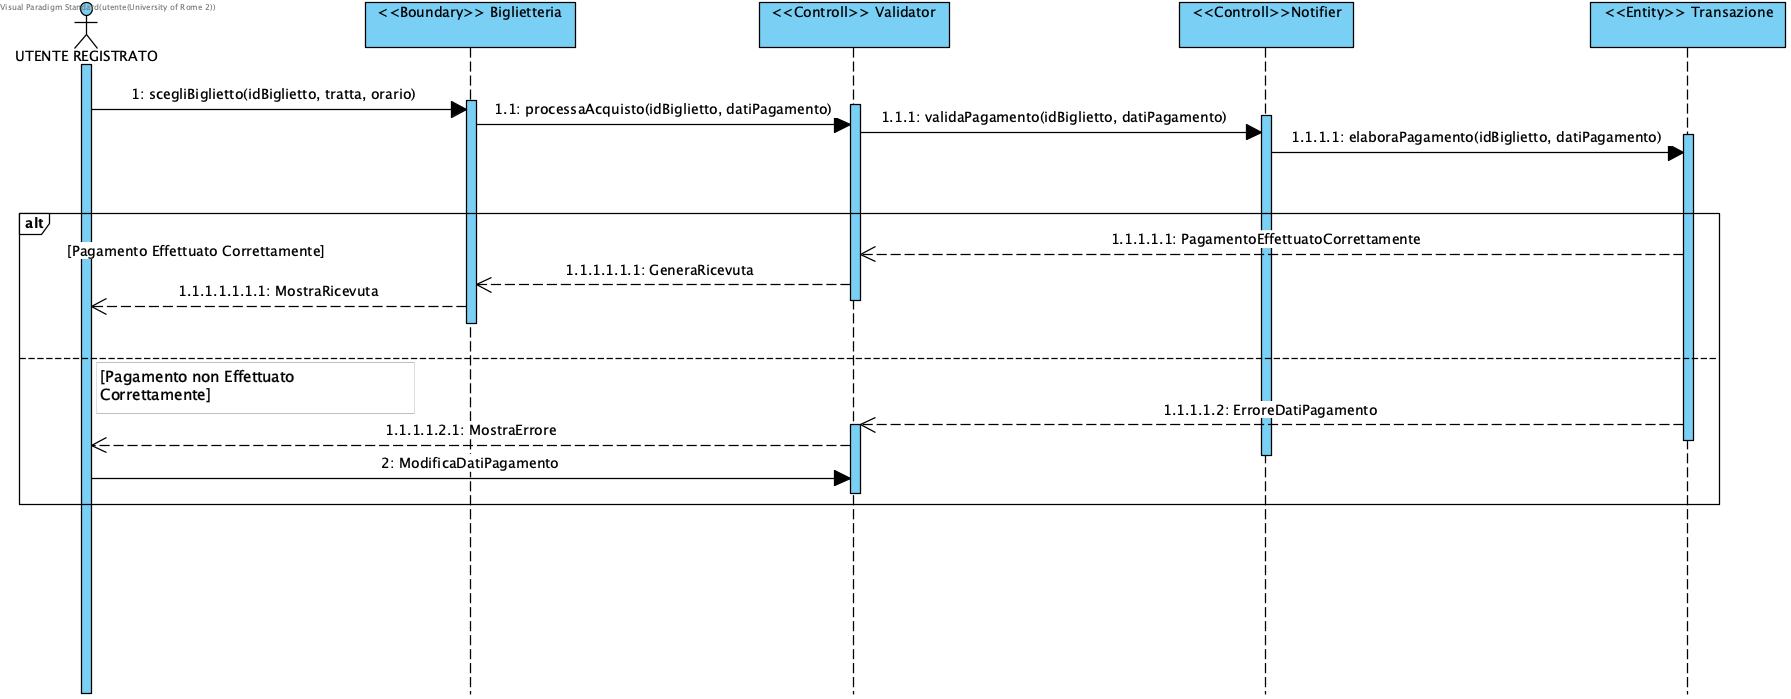
\includegraphics[width=1.0\textwidth]{Sequence Diagram/UTENTE_REGISTRATO_(Pagamento_Biglietto).png}
    \caption{}
    \label{fig:seq_ticket}
\end{figure}
\vspace{1em}
\begin{figure}[H]
    \centering
    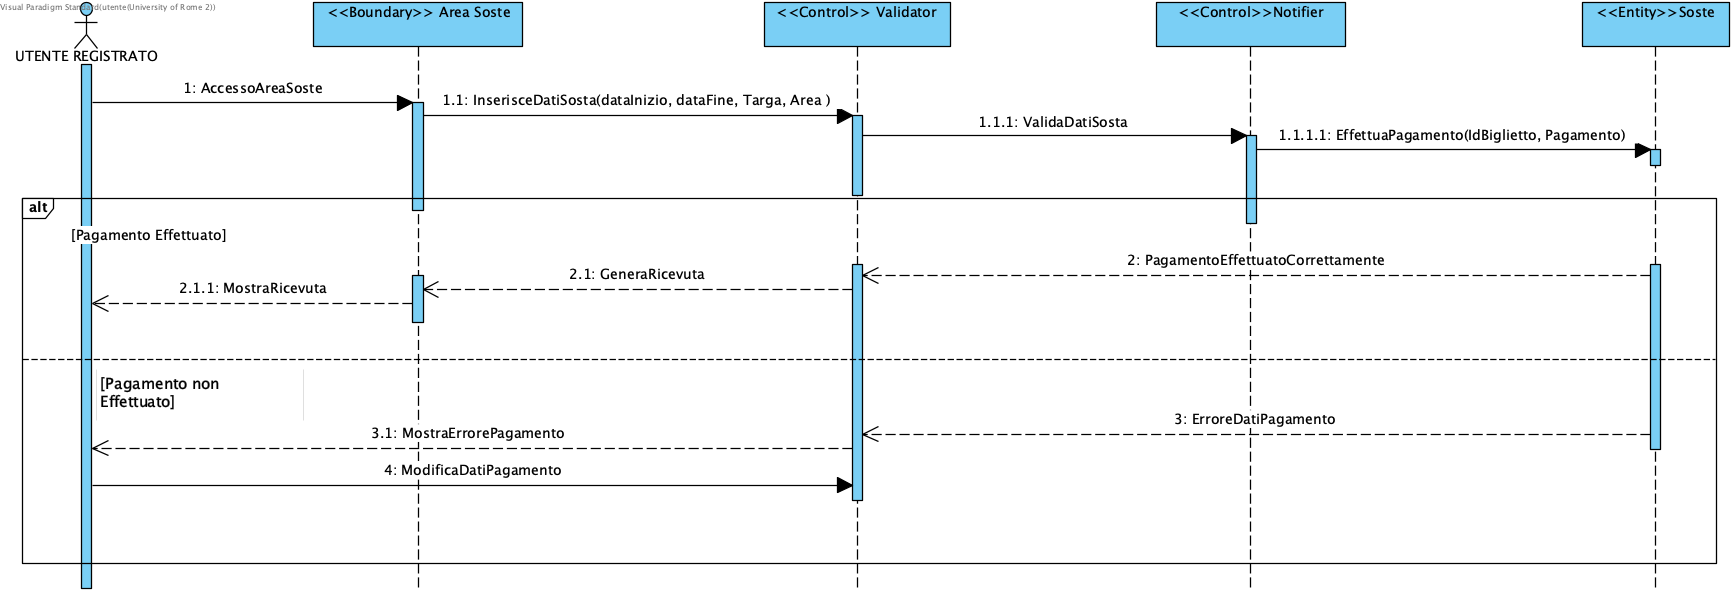
\includegraphics[width=1.0\textwidth]{Sequence Diagram/Pagamento_Soste.png}
    \caption{}
    \label{fig:seq_soste}
\end{figure}
\newpage

\noindent Oltre ai classici servizi di linea, il sistema supporta anche la prenotazione di servizi di trasporto a chiamata, noti come \textit{Demand Responsive Transport} (DRT). Come illustrato nel diagramma di Figura \ref{fig:seq_drt}, a seguito dell'inserimento dei parametri di viaggio desiderati, il sistema ricerca corse compatibili e le propone all'utente, permettendogli infine di selezionare un'opzione ed effettuare la richiesta di presa in carico.

\begin{figure}[H]
    \centering
    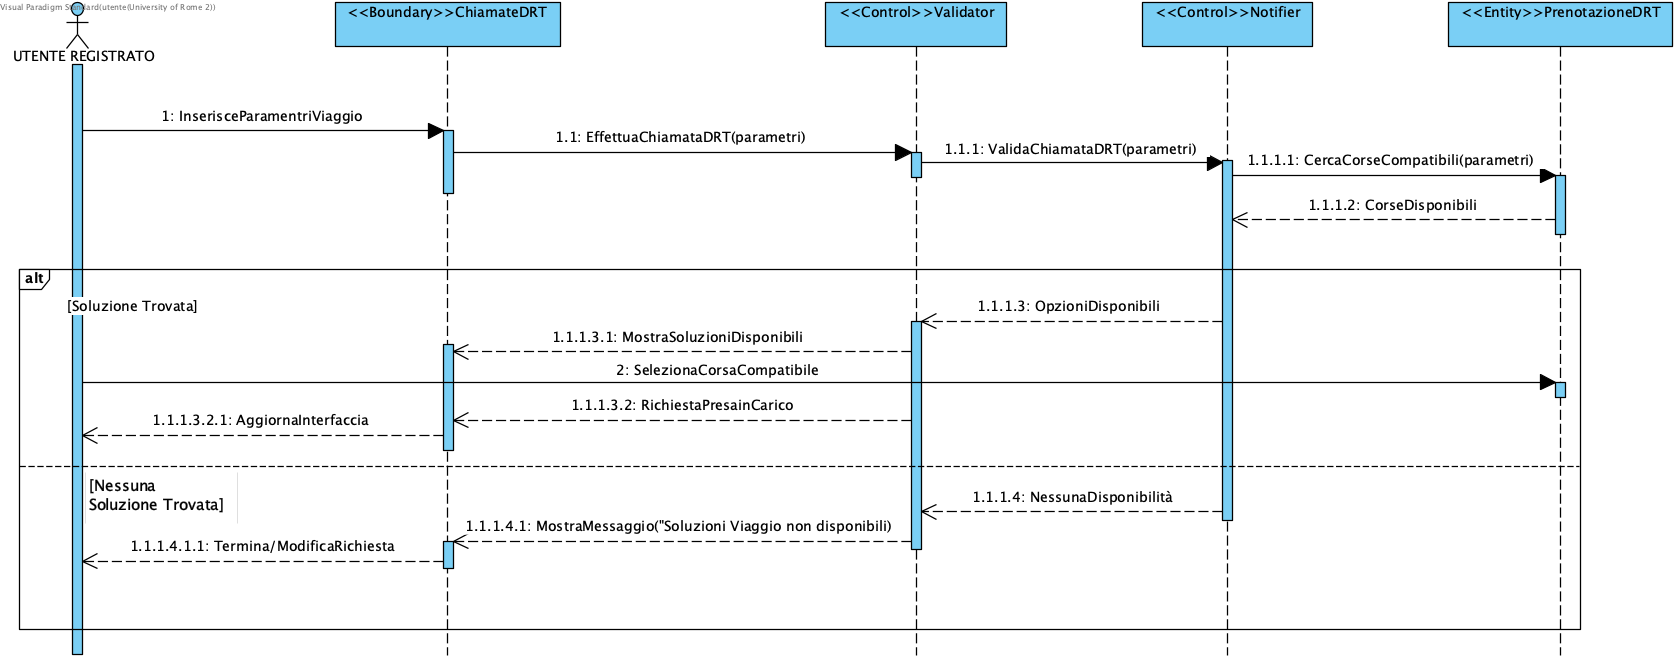
\includegraphics[width=1.0\textwidth]{Sequence Diagram/Utente_Registrato_(Prenotazione_DRT).png}
    \caption{}
    \label{fig:seq_drt}
\end{figure}

\noindent Infine, per garantire all'utente il pieno controllo sulle proprie attività passate, è prevista un'area dedicata alla consultazione dello storico. In quest'ultimo scenario (Figura \ref{fig:seq_storico}), il sistema recupera i dati delle transazioni e dei viaggi pregressi interrogando direttamente l'entità corrispondente e restituendo la lista completa a schermo, o alternativamente notificando l'assenza di dati qualora l'account non presenti attività registrate.

\begin{figure}[H]
    \centering
    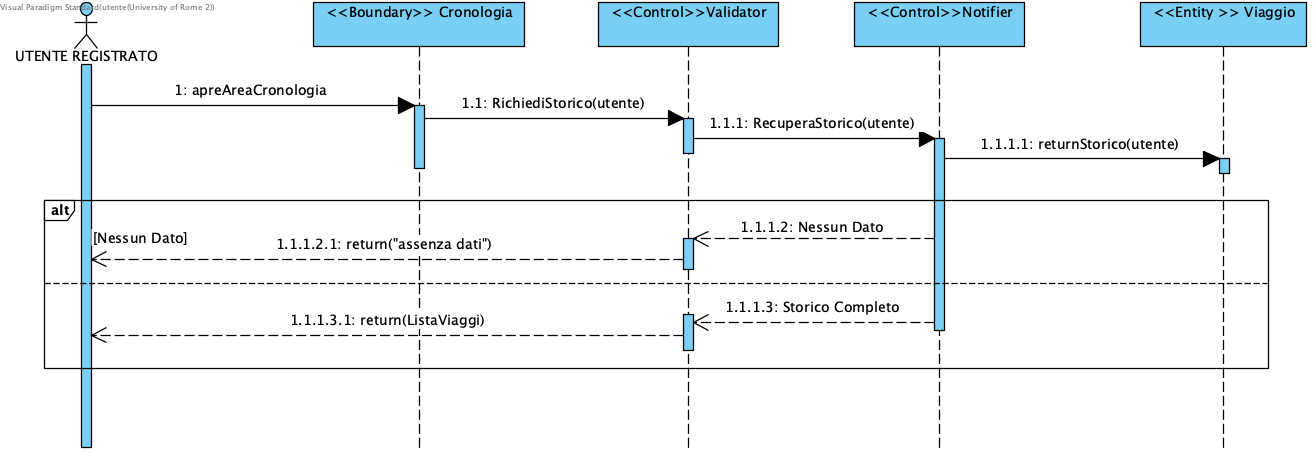
\includegraphics[width=1.0\textwidth]{Sequence Diagram/Utente_Registrato(StoricoUtente).png}
    \caption{}
    \label{fig:seq_storico}
\end{figure}
\newpage

% SEZIONE UTENTE NON REGISTRATO
\subsection*{Sequence dell'Utente non Registrato}
Passiamo ora ad analizzare le azioni che può compiere l'attore \textbf{Utente non Registrato}, cioè chi utilizza l'applicazione senza un profilo attivo. 
\\
L'operazione principale per convertire questo attore in un Utente Registrato è la procedura di registrazione. Come mostrato nella Figura \ref{fig:seq_reg}, l'utente inserisce i propri dati anagrafici nell'apposita area. Le informazioni vengono trasmesse ai moduli di controllo per la validazione: se i dati risultano incompleti o errati, il sistema richiede le opportune correzioni; in caso di dati validi, viene verificata l'unicità del Codice Fiscale interagendo con l'entità Account, per poi confermare la creazione del profilo e abilitare l'accesso ai servizi avanzati.

\begin{figure}[H]
    \centering
    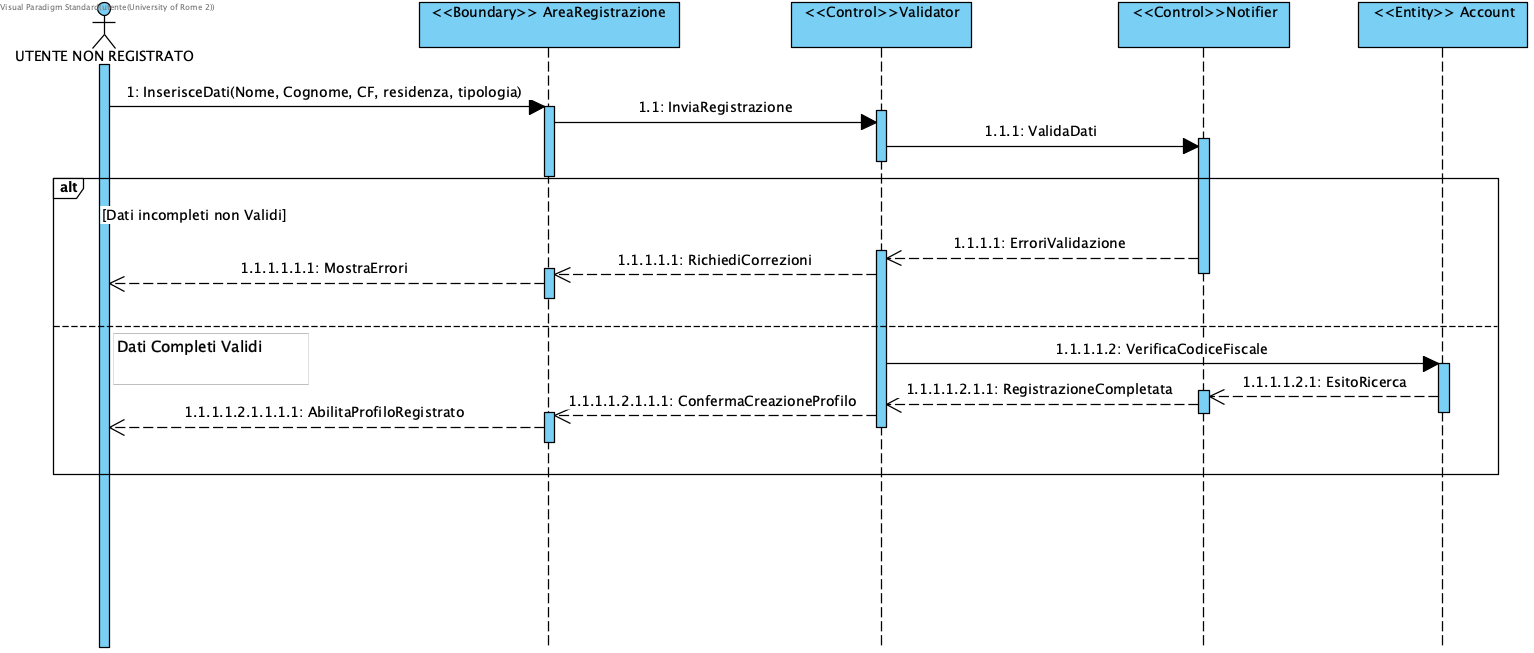
\includegraphics[width=0.8\textwidth]{Sequence Diagram/Utente_non_Registrato(Registrazione).png}
    \caption{}
    \label{fig:seq_reg}
\end{figure}
\noindent
Tuttavia, anche senza aver completato la registrazione, l'utente ha la possibilità di usufruire delle funzionalità pubbliche del sistema, come la consultazione della mobilità (Figura \ref{fig:seq_cons_unreg}). Il flusso è analogo a quello dell'utente registrato: inserendo i parametri di ricerca, il sistema convalida i dati e interroga l'entità Tratta, restituendo infine le soluzioni di viaggio, gli orari e lo stato del servizio, garantendo così un'accessibilità di base alle informazioni sul trasporto.

\begin{figure}[H]
    \centering
    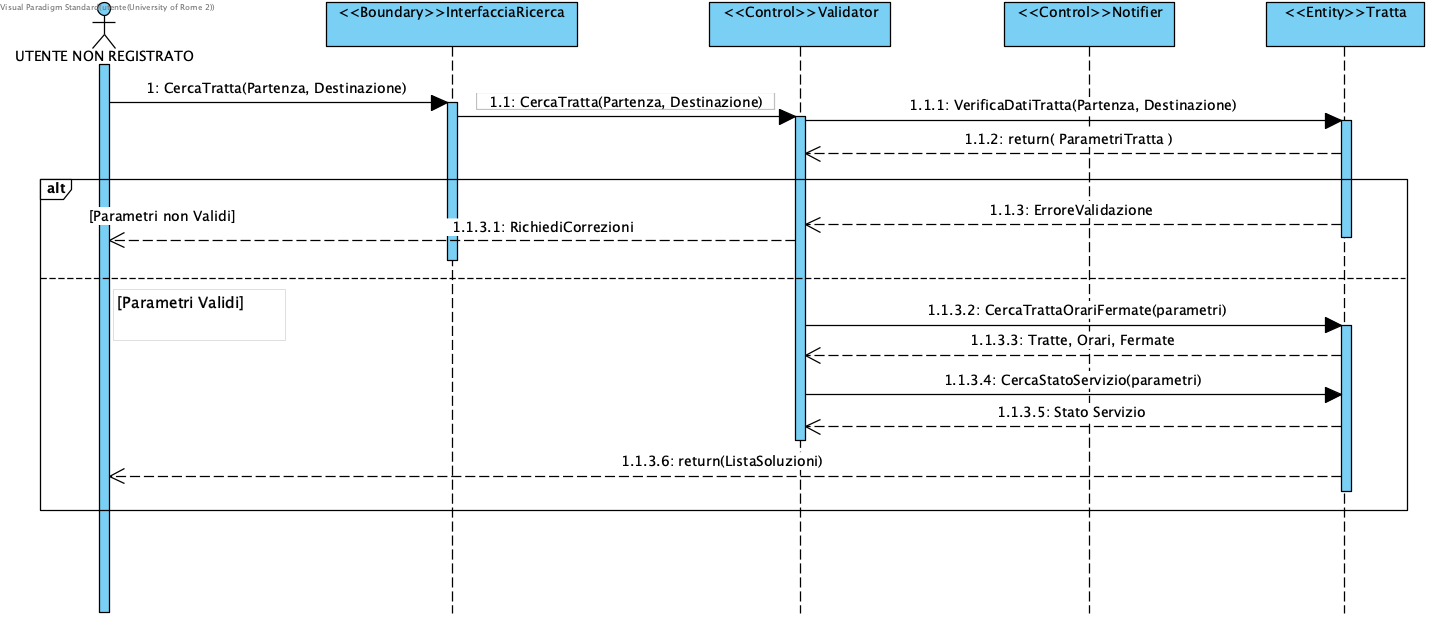
\includegraphics[width=0.8\textwidth]{Sequence Diagram/Utente_non_Registrato(Consultazione_Mobilità).png}
    \caption{}
    \label{fig:seq_cons_unreg}
\end{figure}

% SEZIONE TURISTA
\subsection*{Sequence Turista}
Un ulteriore attore principale all'interno del sistema è il \textbf{Turista}, il quale usufruisce di alcune funzionalità dedicate, pensate per agevolare l'accesso ai servizi di mobilità per periodi limitati o tramite offerte specifiche.
\\
Il primo diagramma di sequenza (Figura \ref{fig:seq_tur_cons}) illustra la procedura di consultazione dei pacchetti speciali. Il Turista accede all'area dedicata alle offerte, innescando una richiesta al sistema che, interfacciandosi con i moduli di controllo, interroga le entità preposte per recuperare le promozioni attive. A seconda dell'esito, il sistema restituisce a schermo l'elenco dei pacchetti disponibili mostrandone i dettagli, oppure notifica l'assenza di offerte attualmente valide.

\begin{figure}[H]
    \centering
    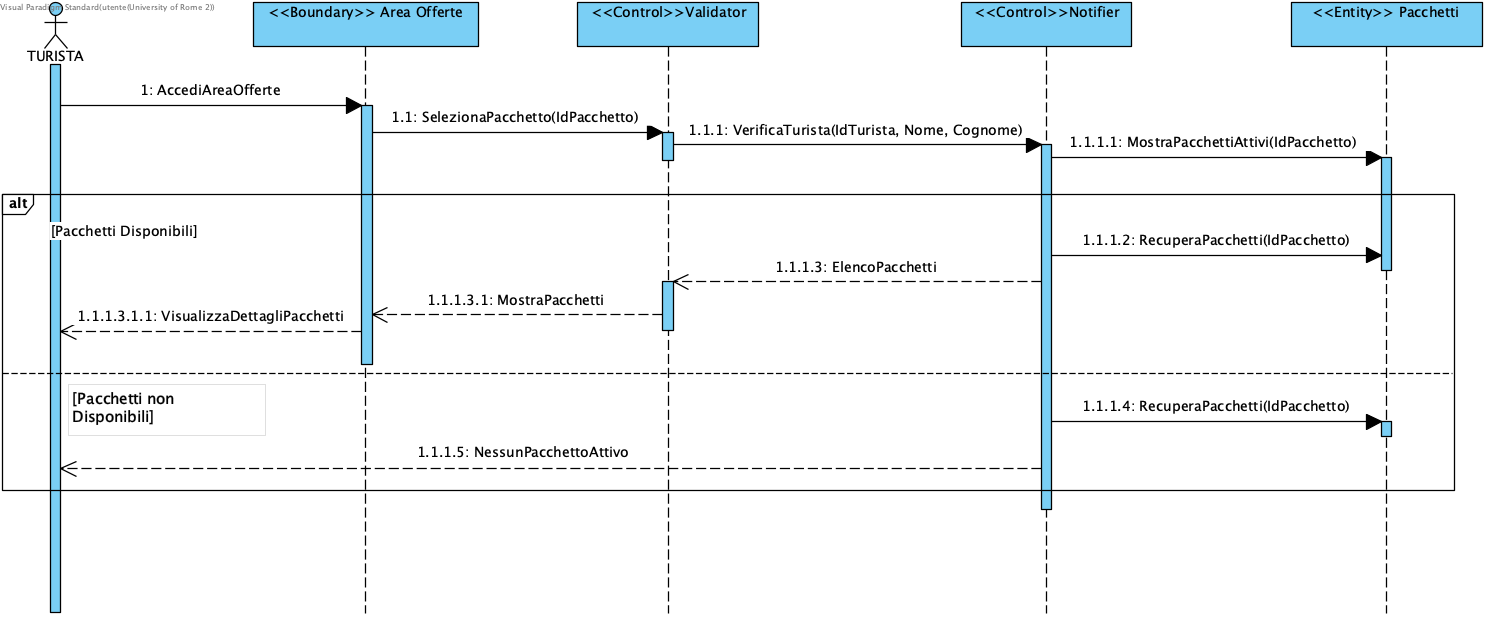
\includegraphics[width=0.8\textwidth]{Sequence Diagram/Turista_(Consultazione_Pacchetti_Speciali).png}
    \caption{}
    \label{fig:seq_tur_cons}
\end{figure}
\noindent Successivamente alla fase di consultazione, il Turista può procedere con l'acquisto di un pacchetto, come descritto nella Figura \ref{fig:seq_tur_acq}. Il diagramma mostra come, partendo dalla selezione del pacchetto desiderato e dal conseguente inserimento dei dati di pagamento, il sistema effettui le necessarie validazioni delegandole ai gestori di controllo. Se la transazione va a buon fine, il sistema genera la relativa ricevuta e conferma l'operazione aggiornando lo stato; in caso contrario, viene restituito un messaggio di errore richiedendo all'utente la modifica e il reinserimento dei dati di pagamento.
\begin{figure}[H]
    \centering
    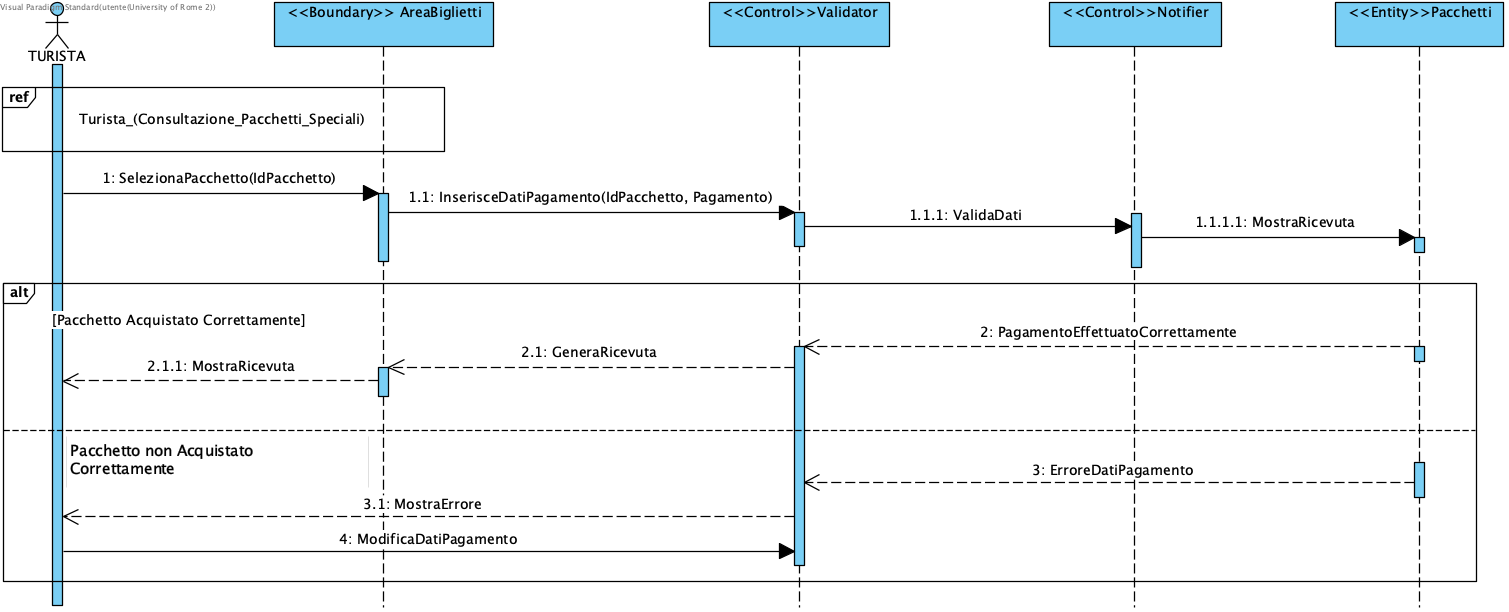
\includegraphics[width=0.8\textwidth]{Sequence Diagram/Turista_(Acquista_Pacchetto_Speciale).png}
    \caption{}
    \label{fig:seq_tur_acq}
\end{figure}


\newpage
% SEZIONE ADMIN
\subsection*{Sequence Admin}
Passiamo ora all'analisi delle operazioni riservate all'attore \textbf{Admin Ente}. 
\noindent Il primo passo fondamentale è l'accesso al sistema. Come illustrato nella Figura \ref{fig:admin_auth}, l'amministratore avvia la procedura di autenticazione. Il flusso prevede controlli decisionali per verificare il possesso di un account e la correttezza delle credenziali inserite. In caso di errore, è prevista la possibilità di recuperare la password o ritentare l'inserimento, iterando il processo fino al raggiungimento dello stato finale di accesso effettuato.
\begin{figure}[H]
    \centering
    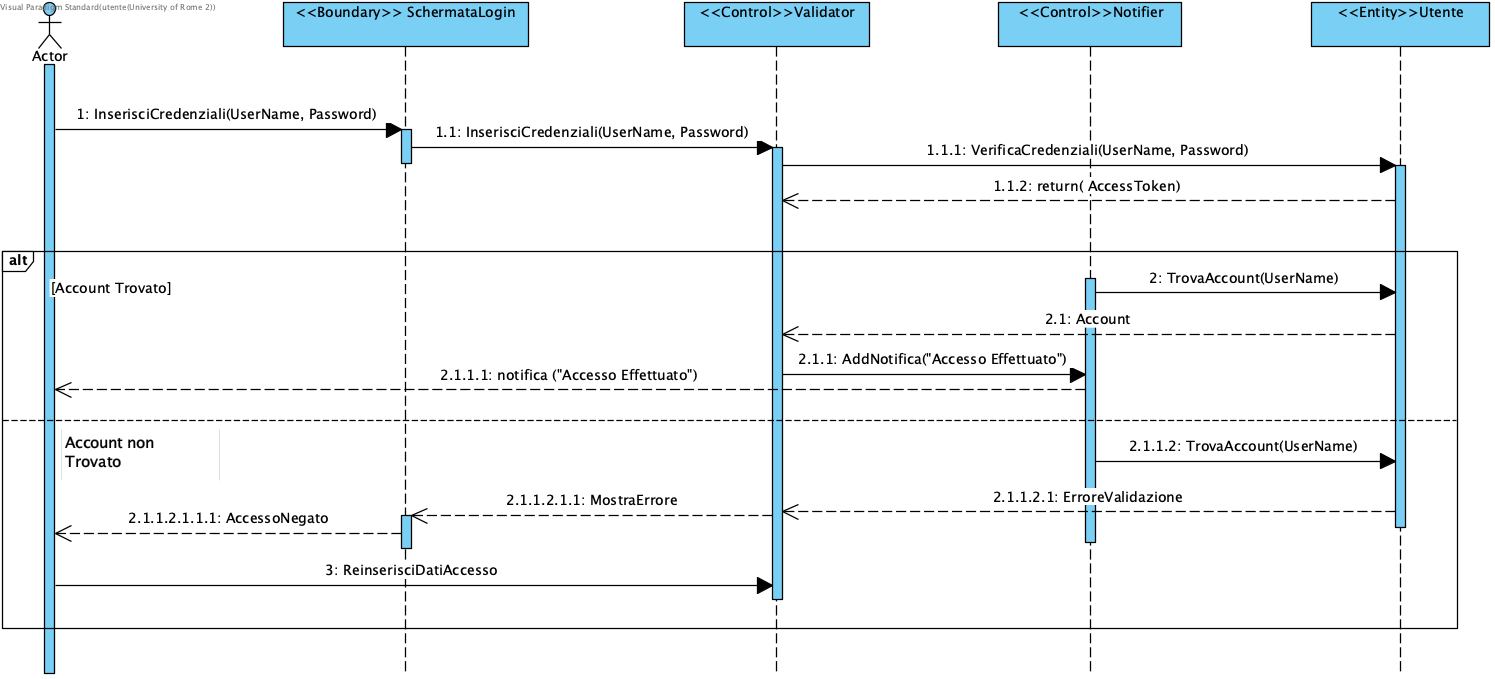
\includegraphics[width=1.0\textwidth]{Sequence Diagram/Admin_Ente_(Autenticazione_Admin).png}
    \caption{}
    \label{fig:admin_auth}
\end{figure}
\newpage
\noindent Una volta completato il login, l'Admin Ente accede all'area riservata, ovvero il Pannello di Mobilità. Il diagramma riportato in Figura \ref{fig:admin_pannello} descrive le molteplici operazioni gestionali a sua disposizione. Dal pannello principale, l'utente può diramare il flusso verso quattro sezioni specifiche: la gestione delle corse, della flotta, delle tariffe e dello staff. Dopo aver effettuato le operazioni richieste (come l'aggiunta, la modifica o la rimozione dei dati), il sistema verifica la correttezza del salvataggio, offrendo infine all'amministratore la scelta se concludere la sessione o tornare al pannello per aprire una nuova sezione.
\begin{figure}[H]
    \centering
    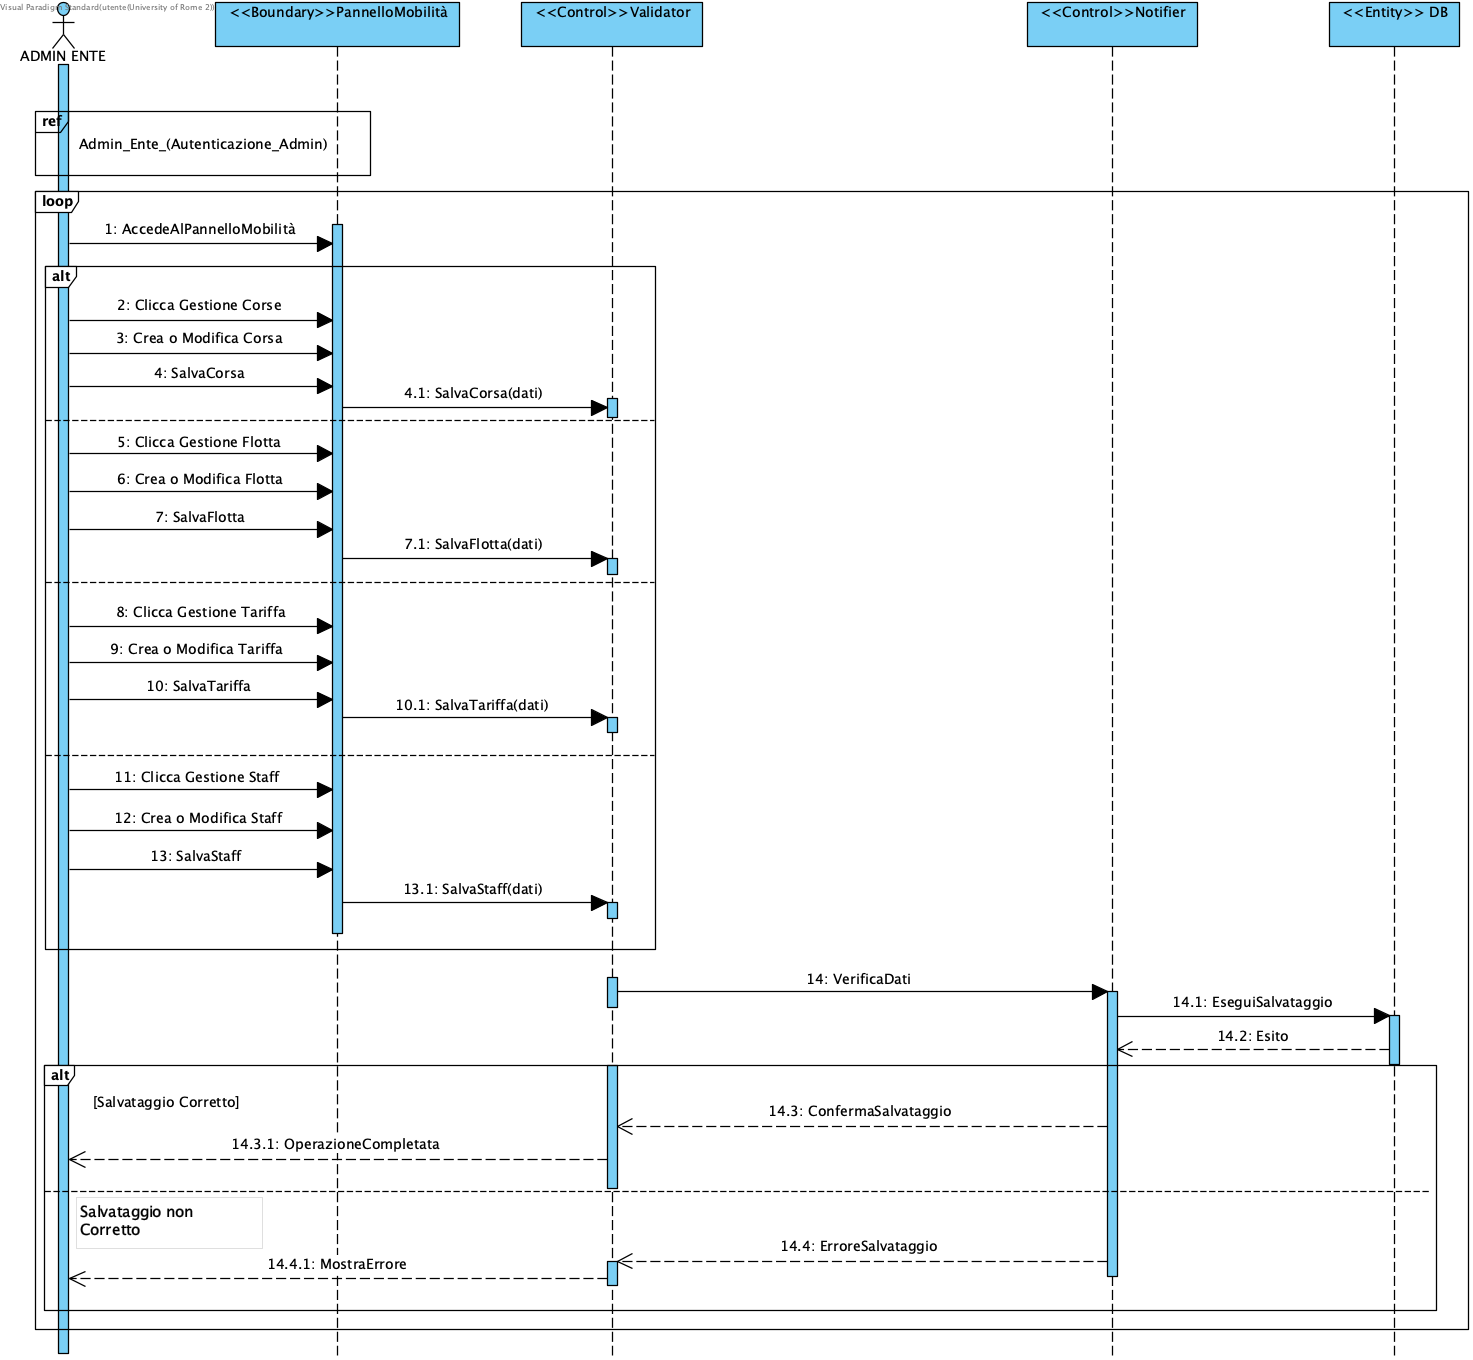
\includegraphics[width=1.0\textwidth]{Sequence Diagram/Admin_Ente_(Gestione_Pannello).png}
    \caption{}
    \label{fig:admin_pannello}
\end{figure}

\newpage
%SEQUENCE OPERAZIONE
\subsection*{Sequence Operatore}
Un ulteriore attore fondamentale per il corretto funzionamento e monitoraggio del sistema è l'\textbf{Operatore}.
\\\\ 
Il primo diagramma (Figura \ref{fig:op_auth}) descrive il processo di autenticazione, essenziale per l'accesso all'area riservata. L'operatore inserisce le proprie credenziali, le quali vengono trasmesse ai moduli di controllo per la verifica interfacciandosi con il database degli utenti. A seconda dell'esito, il sistema autorizza l'accesso generando un token di sessione, oppure notifica l'errore richiedendo un nuovo inserimento.
\begin{figure}[H]
    \centering
    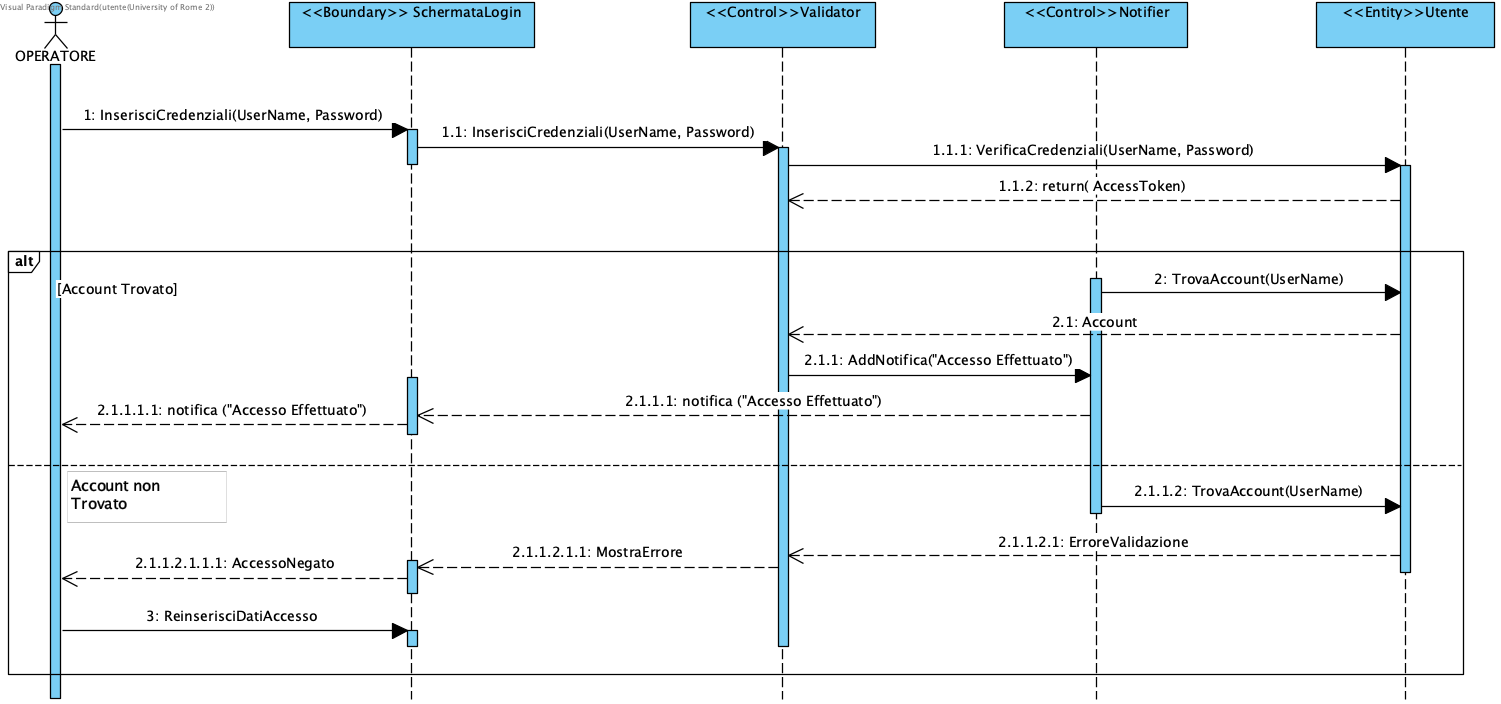
\includegraphics[width=0.8\textwidth]{Sequence Diagram/Operatore_(Autenticazione).png}
    \caption{}
    \label{fig:op_auth}
\end{figure}
\noindent Una delle mansioni principali dell'operatore è la validazione dei titoli di viaggio. Come visibile in Figura \ref{fig:op_verifica}, l'operatore può scannerizzare il QR Code del biglietto tramite il proprio pannello. Il sistema controlla la validità del formato e interroga il database per confermare l'effettiva validità del titolo. Se la scansione automatica fallisce o il formato non è valido, il sistema notifica l'errore richiedendo l'inserimento manuale dei dati.

\begin{figure}[H]
    \centering
    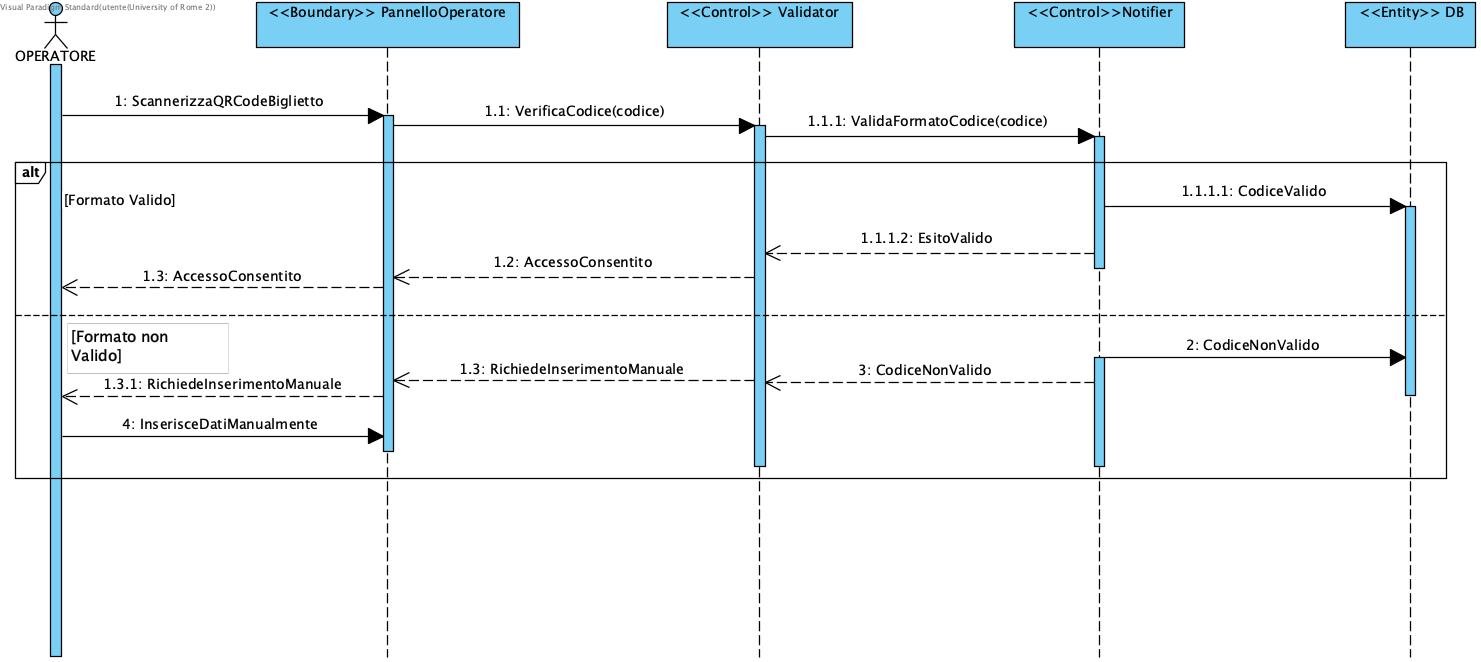
\includegraphics[width=0.8\textwidth]{Sequence Diagram/Operatore_(Verifica_Prenotazioni_e_Titoli).png}
    \caption{}
    \label{fig:op_verifica}
\end{figure}
\newpage
\noindent L'operatore è inoltre incaricato della gestione delle corse DRT (Demand Responsive Transport). Nella Figura \ref{fig:op_drt}, viene illustrato il flusso di presa in carico delle richieste: l'operatore visualizza a schermo le prenotazioni e comunica al sistema la propria decisione (accettazione o rifiuto). I controllori validano i parametri inseriti e aggiornano lo stato della prenotazione all'interno del database.
\begin{figure}[H]
    \centering
    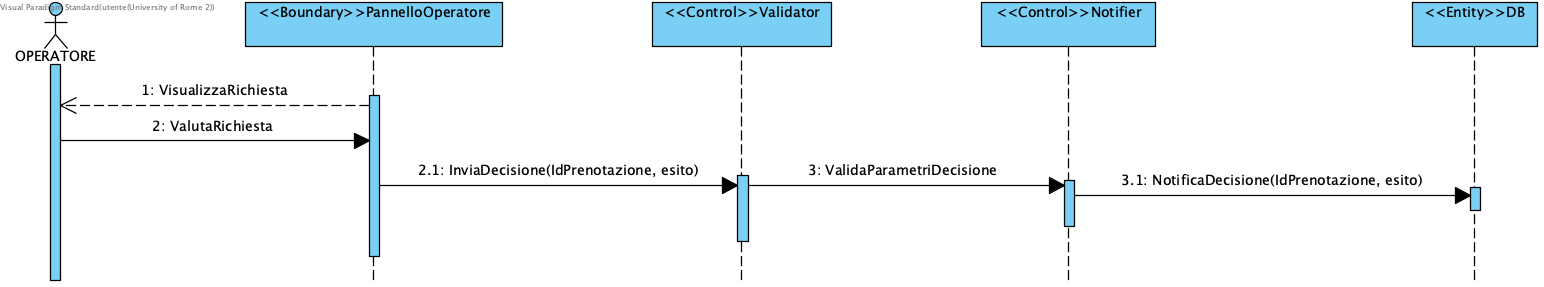
\includegraphics[width=1.0\textwidth]{Sequence Diagram/Operatore_(Gestione_Corse_DRT).png}
    \caption{}
    \label{fig:op_drt}
\end{figure}
\noindent Infine, è prevista la funzionalità di aggiornamento dello stato del servizio, utile per comunicare in tempo reale eventuali ritardi o variazioni. Nel diagramma di Figura \ref{fig:op_stato}, l'operatore seleziona il mezzo e i parametri della corsa per inviare l'aggiornamento. Il backend elabora la richiesta e tenta il salvataggio sul database; l'operazione si conclude con la notifica di successo a schermo o, in caso di anomalie, con un messaggio di errore che invita a ripetere l'inserimento.
\begin{figure}[H]
    \centering
    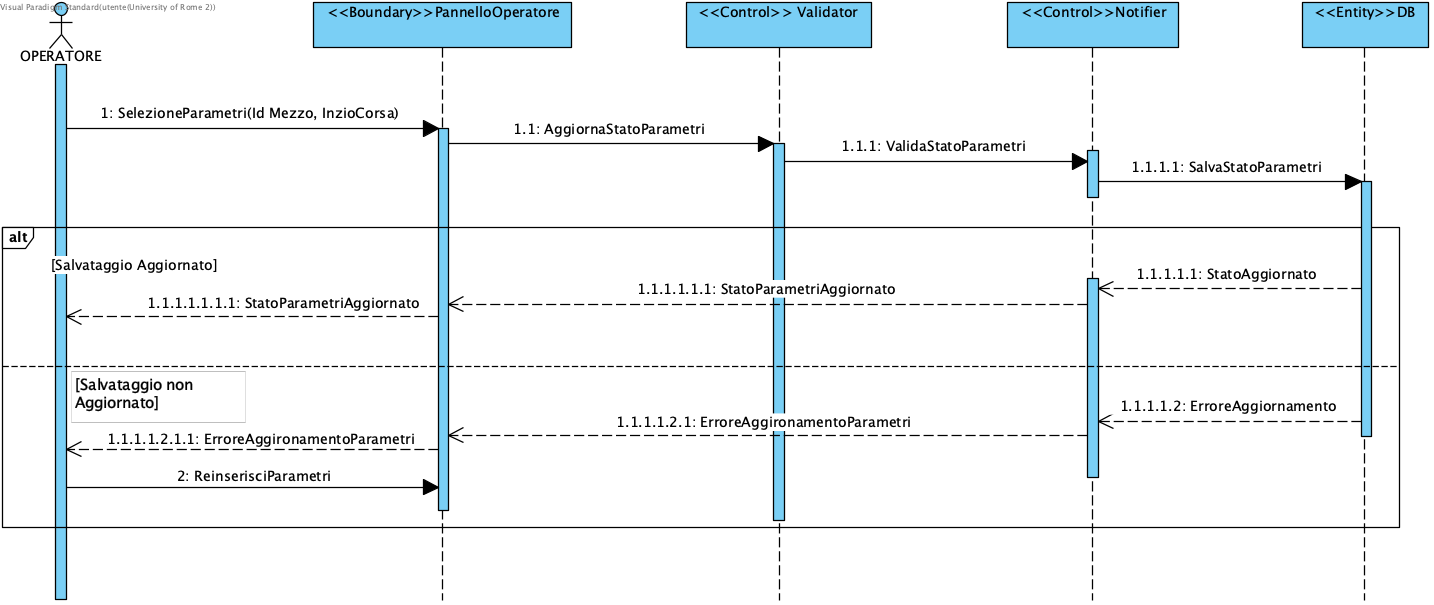
\includegraphics[width=1.0\textwidth]{Sequence Diagram/Operatore_(Stato_Servizio).png}
    \caption{}
    \label{fig:op_stato}
\end{figure}

\newpage
% SEQUENCE FUNZIONARIO COMUNALE
\subsection*{Sequence Funzionario Comunale}
Un altro attore di sistema che andiamo ad analizzare è il \textbf{Funzionario Comunale}. Questa figura istituzionale ha il compito di gestire la viabilità cittadina, inserendo ordinanze e percorsi alternativi che avranno un impatto diretto sui servizi di mobilità.
\\\\
Analogamente agli altri attori, il primo passo per operare all'interno del sistema è l'autenticazione. Come mostrato nella Figura \ref{fig:fc_auth}, il funzionario inserisce le proprie credenziali nella schermata di login. I dati vengono processati dai moduli di controllo per verificarne la validità interrogando il database. In caso di esito positivo, viene garantito l'accesso; in caso contrario, il sistema respinge la richiesta notificando l'errore e invitando a ripetere l'operazione.
\begin{figure}[H]
    \centering
    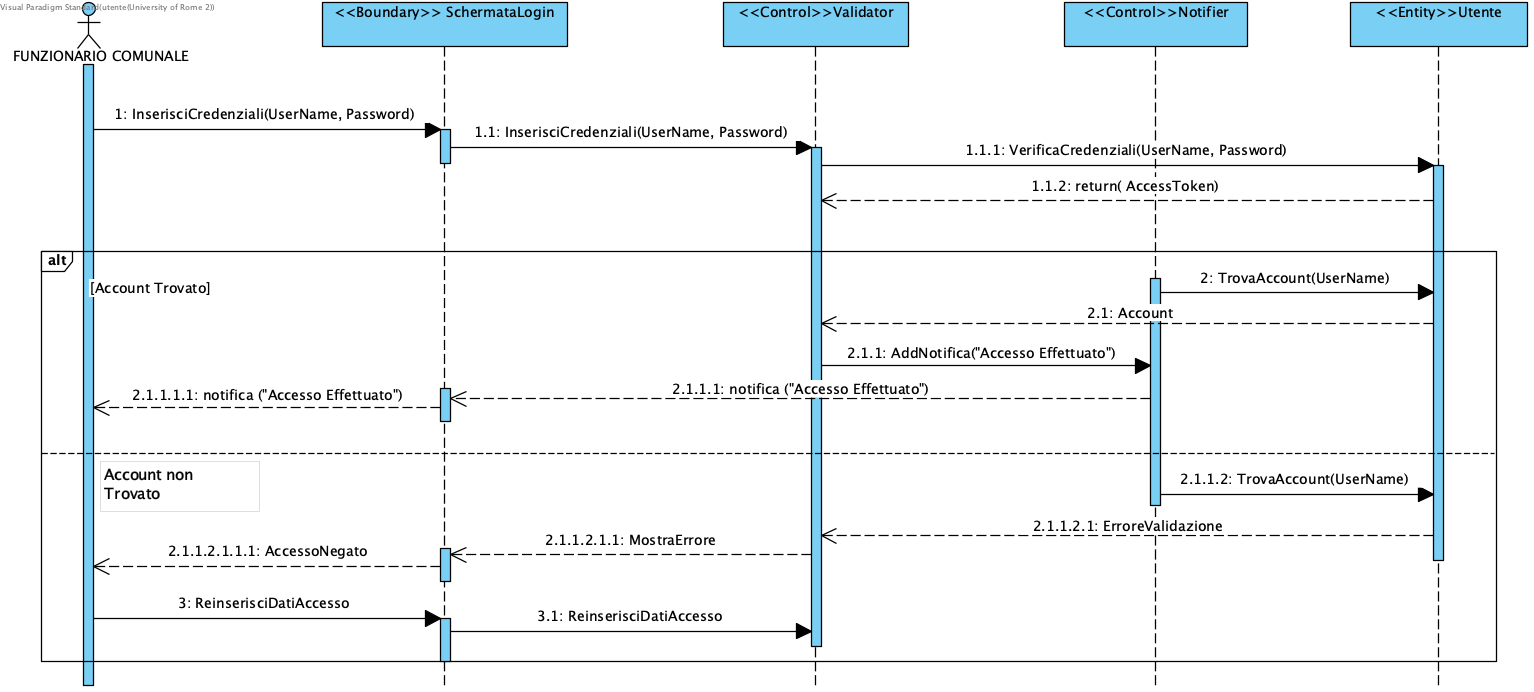
\includegraphics[width=0.9\textwidth]{Sequence Diagram/Funzionario_Comunale_(Autenticazione).png}
    \caption{}
    \label{fig:fc_auth}
\end{figure}
\noindent Una delle funzionalità centrali per questo attore è la gestione delle ordinanze (Figura \ref{fig:fc_ordinanze}). Il funzionario carica il documento ufficiale e seleziona le aree coinvolte tramite l'apposita sezione. Il sistema valida il formato del documento: se non risulta conforme, l'operazione viene interrotta con una richiesta di correzione; se valido, l'ordinanza viene salvata nel database e il sistema restituisce un messaggio di conferma, rendendo l'avviso visibile.
\begin{figure}[H]
    \centering
    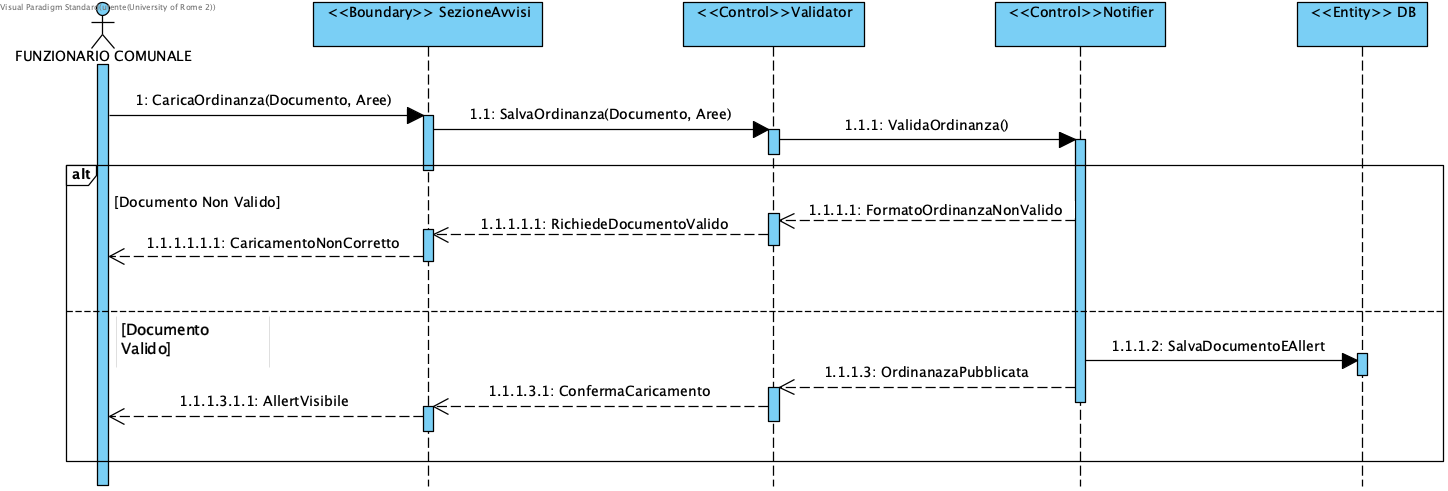
\includegraphics[width=0.9\textwidth]{Sequence Diagram/Funzionario_Comunale_(Gestione_Ordinanze).png}
    \caption{}
    \label{fig:fc_ordinanze}
\end{figure}
\newpage
\noindent A seguito di un'ordinanza, può rendersi necessario modificare la viabilità. Il diagramma di Figura \ref{fig:fc_percorsi} illustra l'inserimento di un percorso alternativo. Richiamando le informazioni dell'ordinanza appena gestita, il funzionario traccia la deviazione; il sistema, dopo aver validato il tracciato, provvede a generare e salvare il nuovo percorso all'interno della base di dati.
\begin{figure}[H]
    \centering
    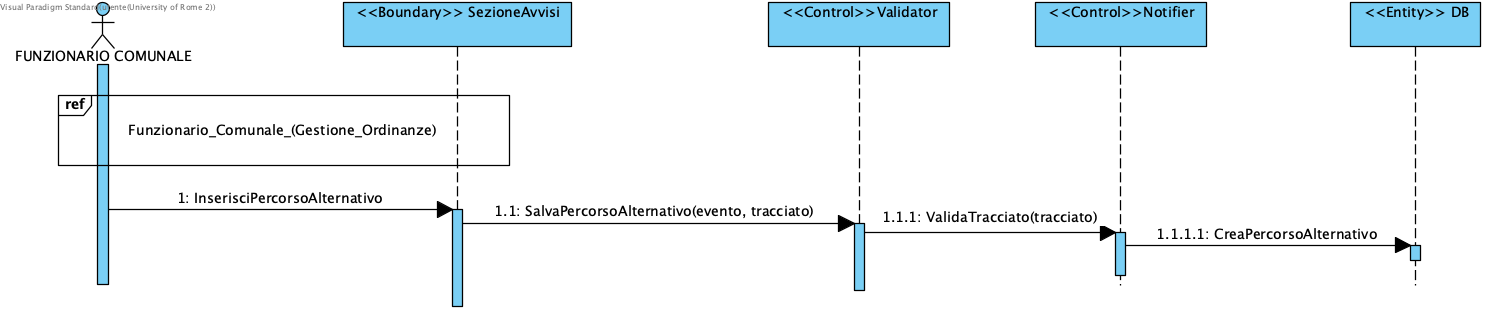
\includegraphics[width=1.0\textwidth]{Sequence Diagram/Funzionario_Comunale_(Gestione_Percorsi).png}
    \caption{}
    \label{fig:fc_percorsi}
\end{figure}
\noindent Infine, per garantire un coordinamento efficace, il funzionario deve poter comunicare le variazioni agli enti terzi. Come visibile nella Figura \ref{fig:fc_notifiche}, l'attore manda un messaggio specificando i destinatari e la relativa ordinanza. I controllori validano il testo e i destinatari, per poi procedere con l'inoltro effettivo. Il sistema conferma al funzionario l'avvenuto invio o segnala un'eventuale mancata ricezione in caso di anomalia.
\begin{figure}[H]
    \centering
    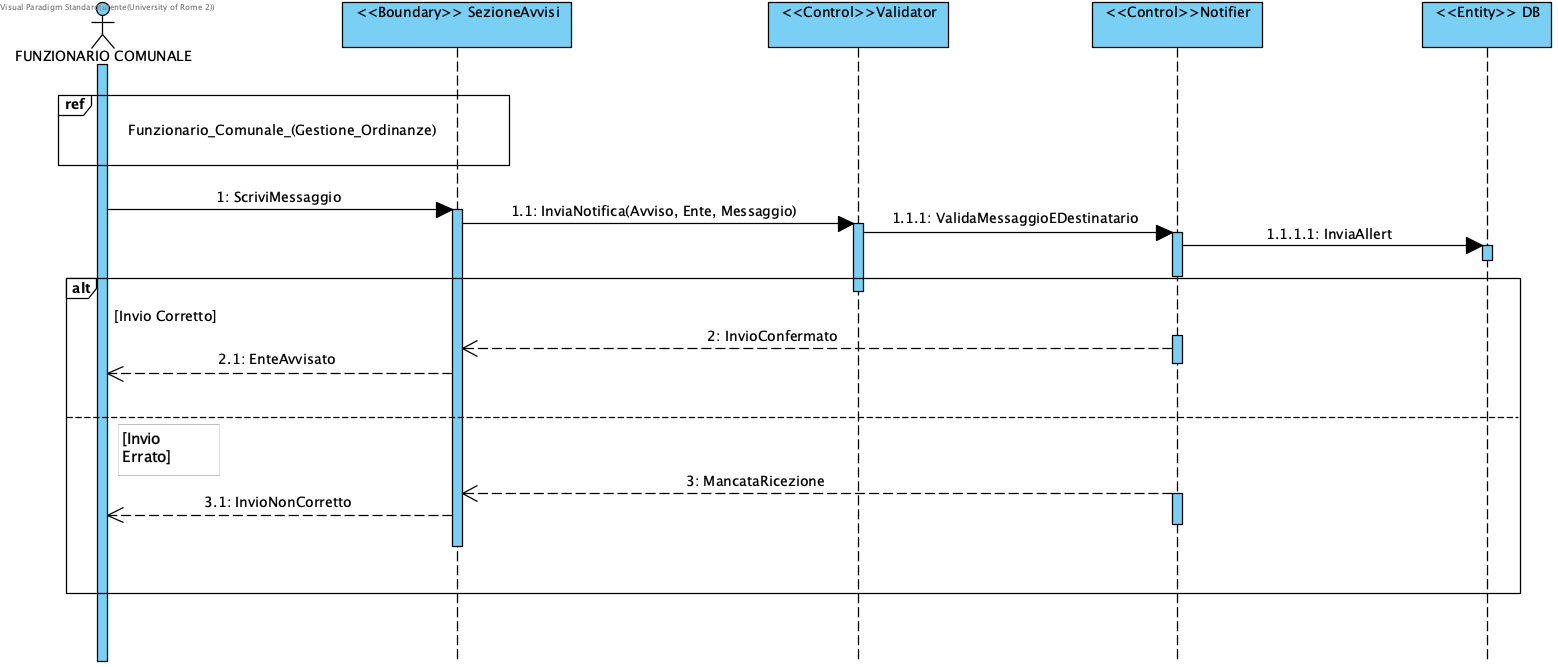
\includegraphics[width=1.0\textwidth]{Sequence Diagram/Funzionario_Comunale_(Notifiche_Enti).png}
    \caption{}
    \label{fig:fc_notifiche}
\end{figure}

\newpage
% SEQUENCE PAYMENT
\subsection*{Sequence Payment}
Infine, ma non per importanza, ci occupiamo della gestione delle transazioni finanziarie, attraverso l'attore \textbf{Payment}. I diagrammi di sequenza seguenti illustrano l'interazione tra l'utente (tramite l'applicazione front-end), il backend MaaS, i gateway di pagamento esterni e il database. 
\\\\
Il processo di elaborazione dei pagamenti (Figura \ref{fig:seq_pagamenti}) si attiva quando l'utente inserisce i propri dati per l'acquisto di un servizio. L'App Front-End inoltra tali informazioni al Back-End MaaS, il quale si fa carico di orchestrare la transazione comunicando in modo sicuro con il Gateway Esterno. In caso di esito positivo, il sistema registra la transazione nel database e restituisce all'utente la ricevuta di pagamento. Qualora i dati risultino non validi o la transazione venga rifiutata, viene registrato il fallimento e notificata a schermo la mancata validazione.
\begin{figure}[H]
    \centering
    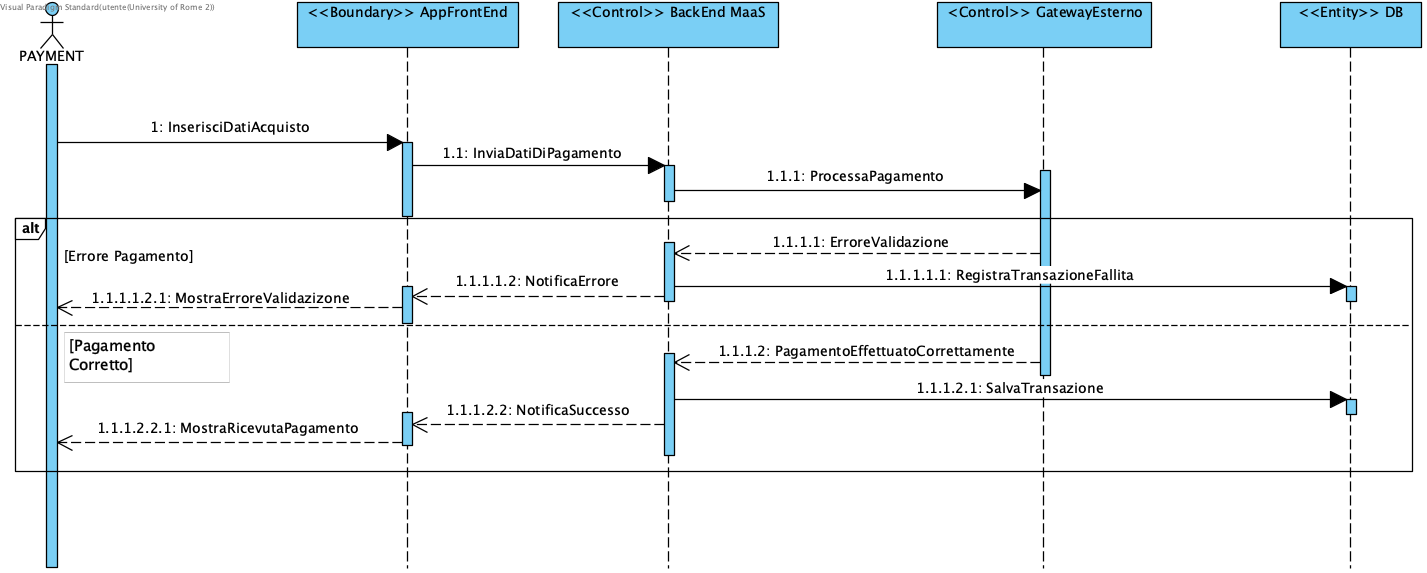
\includegraphics[width=0.9\textwidth]{Sequence Diagram/Payment_(Elaborazioni_Pagamenti).png}
    \caption{}
    \label{fig:seq_pagamenti}
\end{figure}
\noindent
Per quanto riguarda la gestione dei rimborsi, illustrata nella Figura \ref{fig:seq_rimborsi}, prevede una richiesta di rimborso iniziale da parte dell'utente. Successivamente il Back-End MaaS esegue un controllo preliminare interrogando il Database per verificare che la transazione rispetti i termini temporali e le condizioni di rimborsabilità. Se i termini risultano scaduti o non validi, la procedura viene bloccata mostrando un messaggio di negazione. Se i controlli hanno esito positivo, il Back-End inoltra la richiesta al Gateway Esterno per l'erogazione effettiva, concludendo il flusso con l'aggiornamento dello stato nel Database e la visualizzazione della notifica di successo.
\begin{figure}[H]
    \centering
    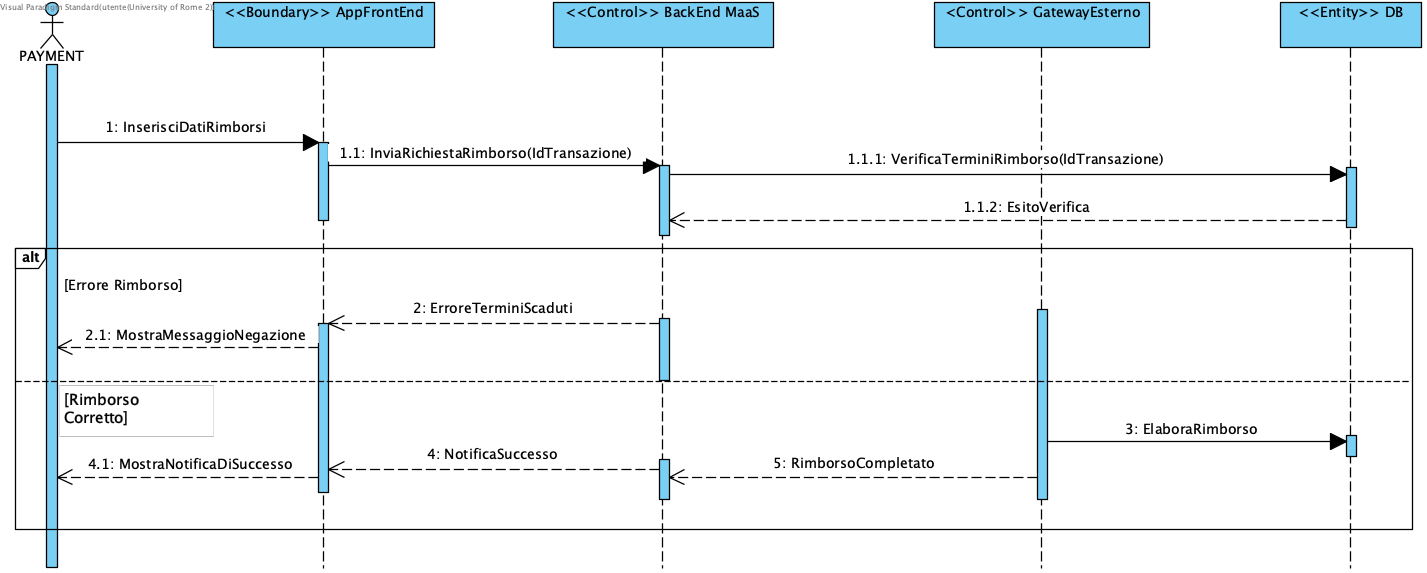
\includegraphics[width=0.9\textwidth]{Sequence Diagram/Payment_(Elaborazione_Rimborsi).png}
    \caption{}
    \label{fig:seq_rimborsi}
\end{figure}

